%% ====== Classe du document ============================================
\documentclass[10pt,a4paper]{article}
%\usepackage[left=1.5cm,right=1.5cm,top=2cm,bottom=2cm]{geometry}

%% ====== Francisation ==================================================
\usepackage[french]{babel}
\usepackage[T1]{fontenc}
\usepackage[utf8]{inputenc}
\usepackage{textcomp}

%% ====== Personnalisation ============================================
\usepackage{fancyhdr}
	\lhead{}
	\chead{Projet MDMA - Rapport L2}
	\rhead{M1 IF 2012-2013}
	\renewcommand{\headrulewidth}{0.3pt}
	\renewcommand{\footrulewidth}{0.3pt}
	\lfoot {}
	\cfoot {- \thepage -}
	\rfoot {}
	\pagestyle{fancy}
\title{Projet MDMA - Rapport L2}
\author{}
\date{}

\usepackage{hyperref}

%% ====== Packages pour le texte ========================================
%\usepackage{soul}
%\usepackage[normalem]{ulem}
%\usepackage{fancybox}
%\usepackage{moreverb}
%\usepackage[table]{xcolor}
%% ====== Packages pour les dessins =====================================
\usepackage{float}
\usepackage{graphicx}
%\usepackage{multicol}
%\usepackage{multirow}
%\usepackage{tikz}
%\usepackage{lmodern}
\usepackage{pict2e}

%% ====== Packages pour les maths =======================================
%\usepackage{amsmath}
%\usepackage{amssymb}
%\usepackage{mathrsfs}
%\usepackage{bussproofs}
%\usepackage[ruled,vlined,french]{algorithm2e}

%%% francisation des algorithmes

%\usepackage[squaren,Gray]{SIunits}
%% ====== Reglages generaux =============================================

\usepackage{titlesec}
	\titleformat{\section}[frame]
	{\normalfont}
	{\filright
	\footnotesize
	\enspace Partie \thesection\enspace}
	{6pt}
	{\bfseries\filcenter}
	
	\titleformat{\subsection}[frame]
	{\normalfont}
	{\filright
	\footnotesize
	\enspace \thesubsection\enspace}
	{6pt}
	{\filcenter}
%	{\titlerule
%	\vspace{.8ex}%
%	\normalfont\itshape}
%	{\thesubsection.}{.5em}{}

	\titleformat{\subsubsection}
	{\titlerule
	\vspace{.8ex}%
	\normalfont\itshape}
	{}{.5em}{}

\titleformat{\chapter}[display]
	{\normalfont\bfseries\filcenter}
	{}
	{1ex}
	{\titlerule[2pt]
	\vspace{2ex}%
	\LARGE}
	[\vspace{1ex}%
	{\titlerule[2pt]}]
	
\parindent=10pt

%\usepackage{makeidx}
%\makeindex
%\newcommand\vect{\overrightarrow}

%\numberwithin{equation}{subsection}


\graphicspath{{img/}}

\usepackage{pdfpages}
%% ================================================================
\begin{document}
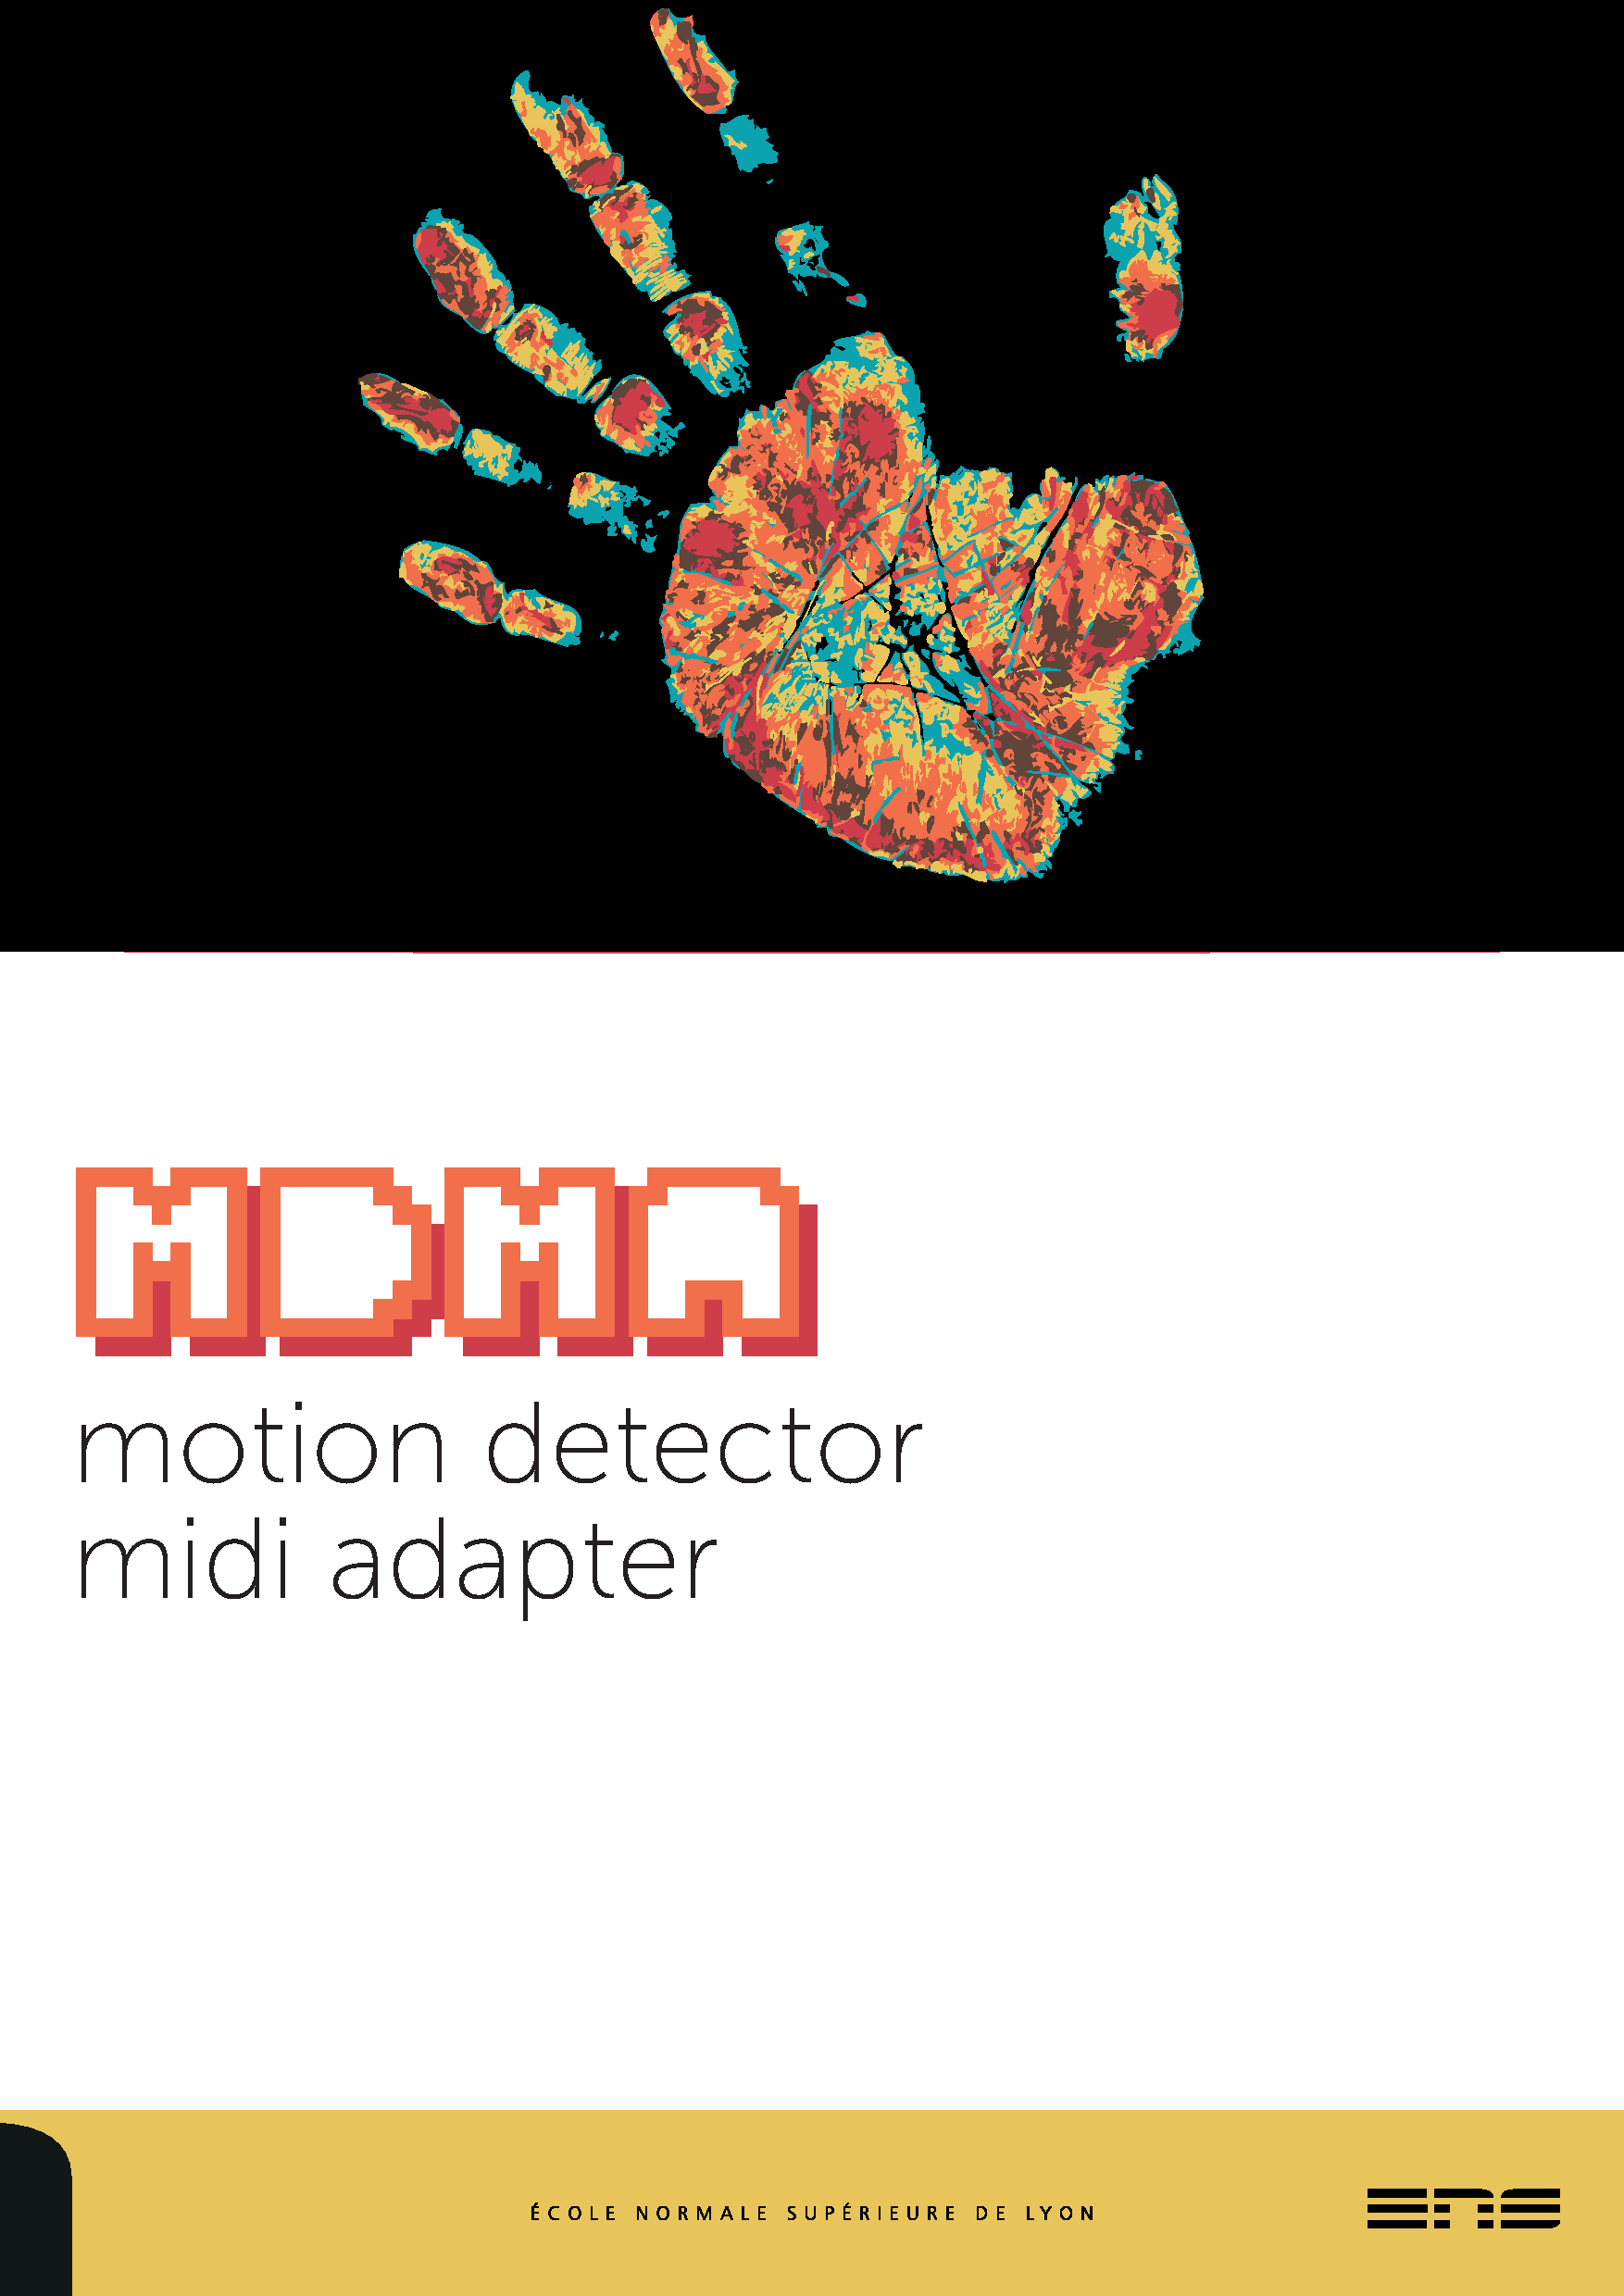
\includepdf[pages=1]{Annexes/Couverture}
\vspace*{\stretch{1}}
\begin{center}
    \emph{Coordinateurs :}\\
    Timothée Bernard, Louis Parlant\bigskip\\
    \emph{Membres du projet :}\\
    Hadrien Croubois, Henri Derycke, Gaëtan Gilbert, Semen Marchuk, Luc Rocher
\end{center}
\vspace*{\stretch{1}}
\newpage
\tableofcontents
\newpage
%% ================================================================
\section{Introduction}
\par Les périphériques traditionnels tels que le clavier et la souris s'avèrent peu adaptés à la composition et l'interprétation de musique par ordinateur. C'est pourquoi toute une gamme de périphériques s'inspirant du materiel de mixage ou d'instruments de musique est aujourd'hui disponible (voir figure~\ref{MIDI_controllers}, garantissant à l'adepte de MAO (\emph{Musique Assistée par Ordinateur}) un confort de travail tout à fait comparable à celui d'un musicien traditionnel. La plupart de ces périphériques utilisent le protocole de communication MIDI et sont donc appellés « contrôleurs MIDI ».
\begin{figure}[h]
    \centering
    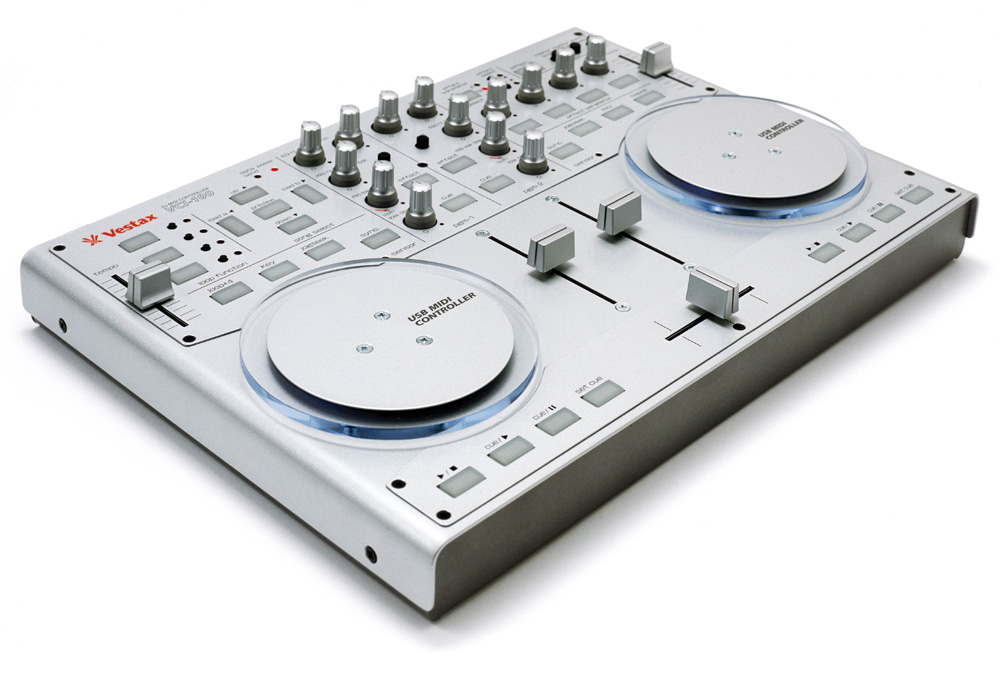
\includegraphics[width=8cm]{tot_controller_01.jpg}
    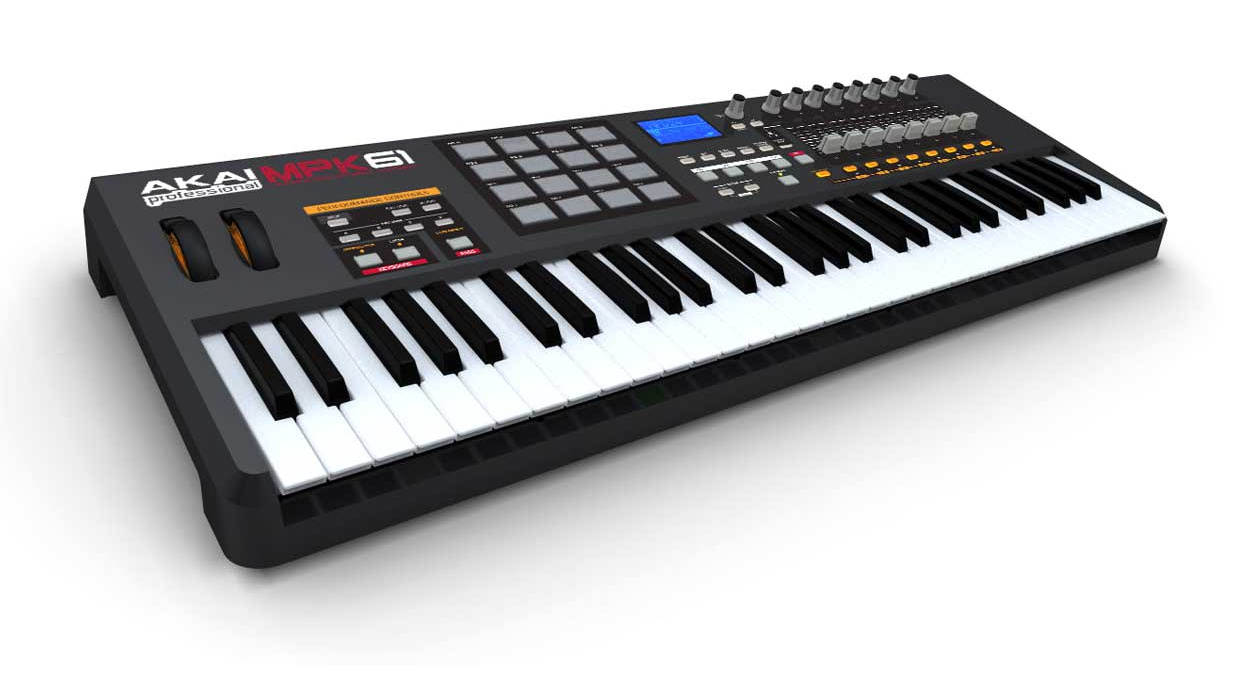
\includegraphics[width=8cm]{tot_controller_02.jpg}
    \caption{Deux exemples de contrôleurs MIDI : le MPK61 d'AKAI (à gauche) et le VCI-100 de Vestax (à droite)}
    \label{MIDI_controllers}
\end{figure}
\par Le but du projet MDMA  – pour \emph{Motion Detection Midi Adapter}  – est de concevoir un contrôleur MIDI reposant sur les mouvements de l'utilisateur filmé par une caméra plutôt que sur la manipulation des nombreux objets physiques (potentiomètres, interrupteurs, surfaces tactiles) qui composent les contrôleurs tradictionnels.
\par Nous avons pris le parti de demander à l'utilisateur un matériel minimal. Une simple webcam suffit à fournir l'image que notre logiciel analyse pour situer les mains. Dans un souci d'efficacité et de précision, nous proposons d'utiliser d'autres types de périphériques d'acquisition. Nous sommes en train de mettre au point une version utilisant la \emph{Microsoft Kinect} et la \emph{Leap Motion} est aussi à l'étude. Ensuite, il s'agit de traduire ces mouvements en commandes MIDI et de pouvoir les exporter vers un autre logiciel.
\par Le travail a été divisé en plusieurs \emph{workpackages} chacun centré sur l'un des aspects fondamentaux du projet :
\begin{itemize}
    \item les spécifications du logiciel (\textbf{Louis Parlant}, Timothée Bernard)
    \item la conception de l'interface graphique (\textbf{Hadrien Croubois}, Luc Rocher)
    \item la gestion des messages MIDI (\textbf{Gaetan Gilbert}, Louis Parlant, Timothée Bernard)
    \item la gestion du flux vidéo et la détection des mains (\textbf{Semen Marchuk}, Henri Derycke, Hadrien Croubois)
    \item la traduction des mouvements des mains en événements (\textbf{Henri Derycke}, Semen Marchuk, Hadrien Croubois)
    \item la communication interne et externe du projet (\textbf{Luc Rocher}, Hadrien Croubois, Timothée Bernard)
    \item l'intégration des différents composants logiciels (\textbf{Hadrien Croubois})
    \item la procédure de test de l'ensemble des fonctionnalités (\textbf{Timothée Bernard})
\end{itemize}
\par Cette découpe accompagnée d'un calendrier a été effectuée afin de répartir le travail intelligemment entre les différents membres du projet de manière à ce qu'ils disposent en permanence d'objectifs définis et des ressources nécessaires à leur réalisation.
\section{Motivations}
\par Pourquoi réaliser un tel projet, et en quoi est-il finalement utile ?\\
MDMA remplit plusieurs objectifs. Tout d'abord, nous nous sommes intéressés à l'idée de transformer des mouvements en musique. Notre but premier était celui-ci, faire de la musique avec des instruments invisibles. Mais nous avons très vite choisi de fournir un outil plus général qu'un instrument de musique. Nous avons donc réalisé un contrôleur qui soit utilisable par des professionnels, répondant à plusieurs attentes liées à la musique assistée par ordinateur :
\par Les adeptes d'informatique musicale recherchent souvent des surfaces de contrôle qu'ils peuvent configurer à leur guise pour créer un outil adapté au plus près à leurs besoins. Notre logiciel est entièrement paramétrable, et nous avons voulu laisser la plus grande liberté possible à l'utilisateur. Pour garantir la polyvalence de notre logiciel, le choix de réaliser un contrôleur MIDI s'est rapidement imposé. Plus qu'un instrument, MDMA peut se brancher sur n'importe quel synthétiseur\footnote{instrument générant des sons à partir de composants électroniques} ou logiciel de musique et contrôler les paramètres que  l'utilisateur choisira.
\par Les contrôleurs MIDI modernes se font de moins en moins encombrants, témoignant d'une demande pour un équipement léger et facile à transporter sur scène. Répondant à ce besoin, MDMA ne nécessite aucun matériel, si ce n'est l'ordinateur du musicien et sa webcam. Et puisque notre projet vise à développer un logiciel libre, l'utilisateur n'aura qu'à le télécharger gratuitement sur notre site.
\par MDMA propose ainsi de remplacer des surfaces de contrôle MIDI onéreuses par un programme facile à utiliser où nos mains deviennent des contrôleurs.
\section{Spécifications}
\par MDMA est multi-plateforme : la version alpha du logiciel fonctionne sous Linux, Windows et OS X, et il est prévu que ce soit le cas pour toutes les versions ultérieures.
\par Le logiciel possède deux composants principaux : un analyseur de flux vidéo qui détecte certains types de mouvements et produit en sortie des signaux MIDI, ainsi qu'un éditeur de configurations.
\par Le flux vidéo, provenant soit d'une webcam soit d'un périphérique \emph{Kinect}, est analysé en temps réel avec une latence non perceptible par l'être humain.
\par La position, la vitesse, l'accélération ainsi que l'état ouverte/fermée de chaque main sont déterminés afin de détecter les mouvements associés à l'envoi de messages MIDI, décris par un évènement.
\par Les événements sont définis à partir de trois types d'élèments virtuels, les faders, les pads et les segments, qui suffisent à simuler tous les éléments physiques d'un contrôleur MIDI habituel (potentiomètres, boutons, etc) si on les configure de différentes manières. Ils correspondent à différentes parties de l'image (voir la figure~\ref{img_spec_01}), les faders et les pads sont des rectangles, les segments des segments de droite (notons que tous ces éléments sont fixes) et c'est l'interaction des mains avec eux qui crée les événements. 
\begin{figure}[h]
\centering
    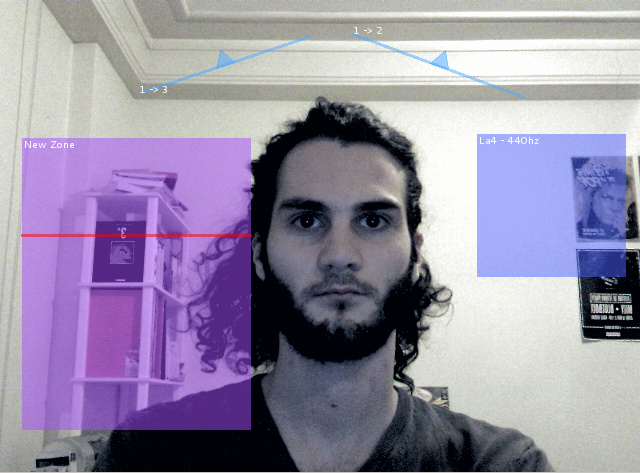
\includegraphics[width=12cm]{img_spec_01.jpg}
    \caption{Affichage de d'un fader (en violet), d'une pad (en bleu foncé) et de deux segments (en bleu clair)}
    \label{img_spec_01}
\end{figure}
\par Les évènements sont de différents types :
\begin{itemize}
    \item pour les faders :
        \begin{enumerate}
            \item le déplacement d'une main fermée dans le fader suivant l'axe horizontal
            \item idem pour l'axe vertical
        \end{enumerate}
    \item pour les pads :
        \begin{enumerate}
            \item l'entrée d'une main dans le pad
            \item la sortie d'une main du pad
            \item l'ouverture d'une main dans le pad
            \item la fermeture d'une main dans le pad
            \item la frappe d'une main dans le pad\footnote{cet évènement n'est pas encore géré par le logiciel}
        \end{enumerate}
    \item pour les segments :
        \begin{enumerate}
            \item le franchissement du segment par une main
        \end{enumerate}
\end{itemize}
\par Il est bien possible de détecter chacun d'entre eux à partir de la position, la vitesse, l'accélération et l'état ouverte/fermée de chaque main aux différents instants successifs.
\par Chacun de ces événements, suivant la configuration utilisée, peut déclencher l'émission d'un signal MIDI ce qui permet de simuler :
\begin{itemize}
    \item un potentiomètre rectiligne ou un pad XY par un fader
    \item un bouton par un segment sensible au franchissement ou par un pad sensible à l'ouverture, la fermeture de la main ou à la frappe.
\end{itemize}
\par Les zones créées par l'utilisateur peuvent être sauvegardées dans un fichier de configuration. Une configuration est une liste d'onglets, qui contiennent une liste de faders, de pads et de segments, chacun associé à sa taille et sa position. Les configurations décrivent aussi comment réagissent ces éléments : à chacun d'entre eux, pour tout évènement qu'il définit peut correspondre un signal MIDI à envoyer ou un changement d'onglet. L'envoi de signaux MIDI permet la fonction première de MDMA, à savoir être un contrôleur MIDI, le changement d'onglet permet d'améliorer l'ergonomie du logiciel en définissant en quelque sorte plusieurs espaces de travail (voir figure~\ref{chgt_onglet}).
\begin{figure}[h]
    \centering
    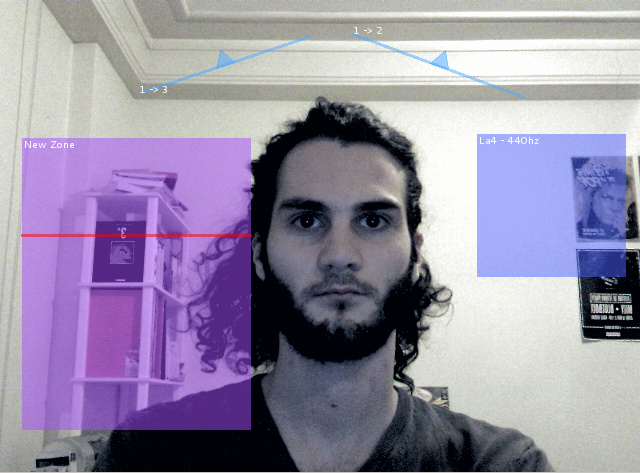
\includegraphics[width=8cm]{img_spec_01.jpg} 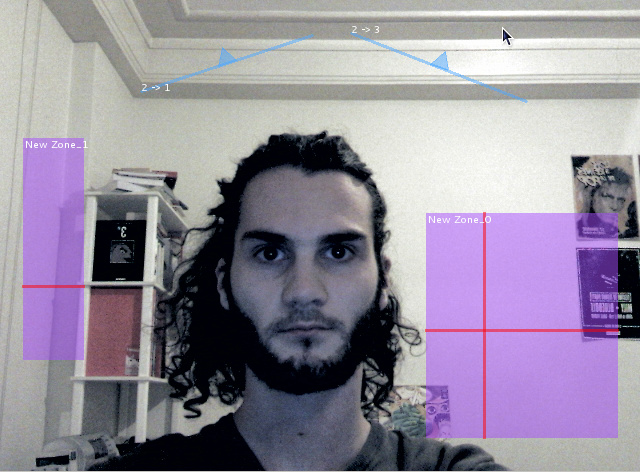
\includegraphics[width=8cm]{img_spec_02.jpg}
    \caption{Dans cette configuration, les deux images illustrent les onglets 1 et 2 contenant chacun des objets différents ; le passage d'un onglet à l'autre s'effectue en traversant l'un des segments}
    \label{chgt_onglet}
\end{figure}
\par Les signaux MIDI sont transférés par l'intermédiaire de ports MIDI, les ports d'entrée sont faits pour recevoir des messages, les ports de sortie pour en envoyer. MDMA peut au choix créer un port de sortie auquel peuvent se connecter d'autres logiciels qui y récupèrent les messages envoyés par MDMA, ou bien se connecter au port d'entrée d'un autre logiciel et y envoyer ses messages.
\par Le logiciel MDMA se présente à l'utilisateur sous la forme d'une unique fenêtre affichant :
\begin{itemize}
    \item un menu général (proposant de charger et de sauvegarder une configuration)
    \item une boite affichant des informations sur la configuration utilisée
    \item un flux vidéo de contrôle représentant l'image acquise par la caméra sur laquelle se surimpression les différents faders, pads et segments de l'onglet en cours dans la configuration utilisée.
\end{itemize}
Un code de couleurs et d'opacités sur les zones et les segments permet de mettre en évidence la détection des événements.
\section{Design Interface \& Intégration}
\subsection{Objectifs}
\par La partie "Design Interface" a pour objectif de mettre au point et d'implémenter l'interface graphique ainsi que de penser a l'interconnexion de l'interface avec l'ensemble des composants du logiciel. Il s'occupe en plus de la gestion des configurations décrites par l'utilisateur, qu'il s'agisse de leur paramétrage via les différentes fenêtres ou de la partie chargement/enregistrement. La connaissance de l'état d'avancement des différents groupes participants au projet permet de définir efficacement les formats de configuration ainsi que de penser les flux de données nécessaires a l'affichage au cœur de la structure du programme.
\par Le \emph{workpackage} "Design Interface" anticipe à ce titre une part de l'intégration.
\subsection{L'interface}
\par L'interface en elle même est écrite a l'aide du designer de fenêtre de \emph{QtCreator}\footnote{QtCreator - \url{http://doc.qt.digia.com/qtcreator/index.html}}.
\par La fenêtre principale permet, en plus de la visualisation de l'image acquis par la webcam de charger et sauvegarder différentes configuration ainsi que d'avoir un résumé des différentes zones définies. Ces zones peuvent être crées en cliquant sur la vidéo, modifiées et supprimées.
\begin{figure}
    \centering
    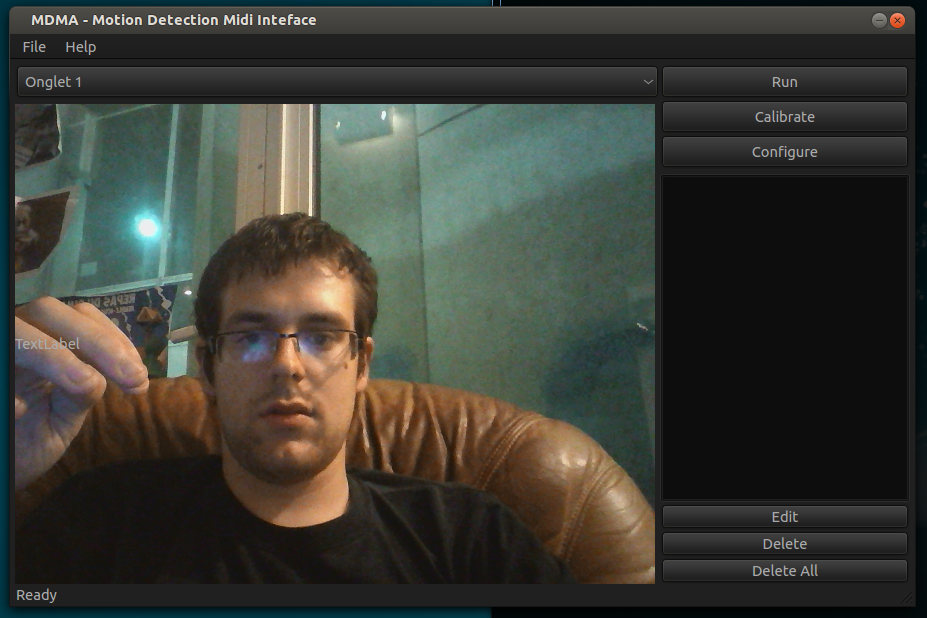
\includegraphics[width=11cm]{design_window.png}
    \caption{La fenêtre principale de l'interface}
\end{figure}
\par L'ouverture d'une nouvelle configuration ou la fermeture du programme alors que la configuration actuelle a été récemment modifiée demande a l'utilisateur de sauvegarder la configuration actuelle.
\par Un bouton "Calibrate" lancera une procédure de calibration, de même que le bouton "Configure" ouvre une fenêtre permettant de choisir différentes options (caméra si plusieurs sont disponibles, port MIDI...).
\par Un bouton "Run" lance le programme. Une fois lancé, la configuration n'est plus éditable (les différents boutons sont désactives). Seul le bouton "Run", renommé en "Stop", reste actif et permet d'arrêter le programme.
\par Enfin, un bouton "Configure" permet d'ouvrir la fenêtre de configuration. Cette fenetre permet notament la gerestion les ports midi ainsi que celle des peripheriques de pointage (hand tracking / souris)
\subsection{Intégration}
\par L'intégration des composants provenant des différentes parties du projet a commencé dès lors que ces derniers avaient des composants qu'ils jugeaient fonctionnels. Cela a permis de tester en flux tendu un maximum de ces composants ainsi que d'adapter l'interface aux besoins ponctuels.
\par Des features entieres ont ainsi été produites pour répondre à ces besoin. On pensera notamment à la gestion de la souris comme troisième main, initialement prévu pour tester les zones alors que le handtracking n'était pas fonctionnel, et qui permettent aujourd'hui de compléter l'expérience intéractive.
\par Une autre conséquence de cette phase d'intégration dynamique a été l'évolution des structures de données afin de répondre au mieux aux besoins des features. La plus marquante a probablement été le découpage de la configuration en deux parties, 
\begin{itemize}
    \item Un singleton, contenant toutes les variables d'environnement propre à la session et ne pouvant etre sauvegarder (pointeur vers l'interface graphique, etat de la calibration, port midi actif ...)
    \item Une sous configuration, réduite aux seules variables à enregister (zones, adresse du fichier) qui peut être serializé/parsé et qui rend ainsi possible l'existence de fichiers de sauvegarde.
\end{itemize}
\par L'évolution des descripteurs de zones aillant modifié la structures des données à enregistrer, l'ajout d'un numero de configuration a été nécessaire afin de s'assurer de la bonne compatibilité du fichier de configuration chargé par l'utilisateur.
\par Aujourd'hui la structure de données, qui permet l'interaction du "front-end" (détection des mouvements), du "middle-end" (gestion des zones) et du back-end (envoi des signaux midi) nous semble assez modulable et évolutive pour envisager sereinement l'ajout d'options au "front-end", telles que la gestion de peripheriques comme la Kinect, tout en assurant une entiere compatibilité (aussi bien en terme de fonctionalité que de fiabilité) du reste du programme.
\section*{OpenCV Interface}
\subsection*{Introduction}
\par Une partie fondamentale du fonctionnement de MDMA est la détection des mains de l'utilisateur sur les images fournies par sa webcam, et à partir de là la détermination des différents paramètres physiques servant à l'envoi de messages MIDI (la position des mains, leur vitesse, leur accélération ainsi que leur état ouverte/fermé). La spécification du logiciel exprime explicitement la possibilité pour l'utilisateur d'utiliser MDMA sans matériel autre qu'une simple webcam et l'ordinateur lui même.
\subsection*{Conditions de fonctionnement}
\par Après avoir considéré certaines contraintes pour assurer la reconnaissance des mains, l'équipe de ce \emph{workpackage} a décidé d'utiliser des gants noirs. Les tests ont montré que la reconnaissance des mains avec de tels gants est efficace sous les hypothèses suivantes :
\begin{itemize}
    \item le fond ne contient pas d'objets foncés
    \item le vêtement d'utilisateur est notablement plus clair que les gants, qui doivent être très foncés (de préférence noirs)
    \item l'éclairage est suffisant
\end{itemize}
\par Du point de vue logiciel, le module nécessite que la bibliothèque OpenCV soit installée sur le système.
\par Comme extension du projet initial, nous sommes en train de développer une version de notre logiciel fonctionnant avec une \emph{Microsoft Kinect}. L'utilisation de ce périphérique, parce qu'elle implique des frais de part de l'utilisateur, sera toujours optionnelle. Cependant l'implémentation de cette possibilité est profitable pour les utilisateurs les plus exigeants car permet une reconnaissance des mains bien plus précise.

\subsection*{Algorithme développé}
\par L'algorithme de détection des mains par webcam est implémenté de manière multi-plateforme à l'aide de la bibliothèque OpenCV qui facilite la réalisation des opérations de base sur les images : capture de l'image, opérations avec les canaux, érosion, dilatation et autres.
\paragraph{Structure de l'algorithme}
\begin{itemize}
    \item  Calibration du système : l'utilisateur place les mains dans des zones dessinées à l'écran. Après cela le système fixe $L'$ égal à l'éclairage du point hors de ces zones le plus sombre. $L=L'-\Delta$ devient le seuil critique de luminosité. On utilise pour la calibration 2 images : celle avec les mains ouvertes et celle avec les mains fermées. Après la détermination du seuil de luminosité on fait un tour de la boucle présentée ci-dessous et on calcule la surface des mains pour les deux images. La moyenne de ces valeurs définit le seuil de la surface utilisé pour dire si la main est ouverte ou fermée. Après cette étape la boucle principale de fonctionnement se déroule.
    \item Commencement de la boucle : capture de l'image.
    \item Conversion RGB vers Niveau de Gris (luminosité calculée avec la formule: $Y'=0.299 \ cdot R + 0.587 \cdot G +  0.114 \cdot B$, formule largement utiisée dans de nombreux logiciels graphiques). 
    
		\begin{figure}[h!]
    		\centering
    		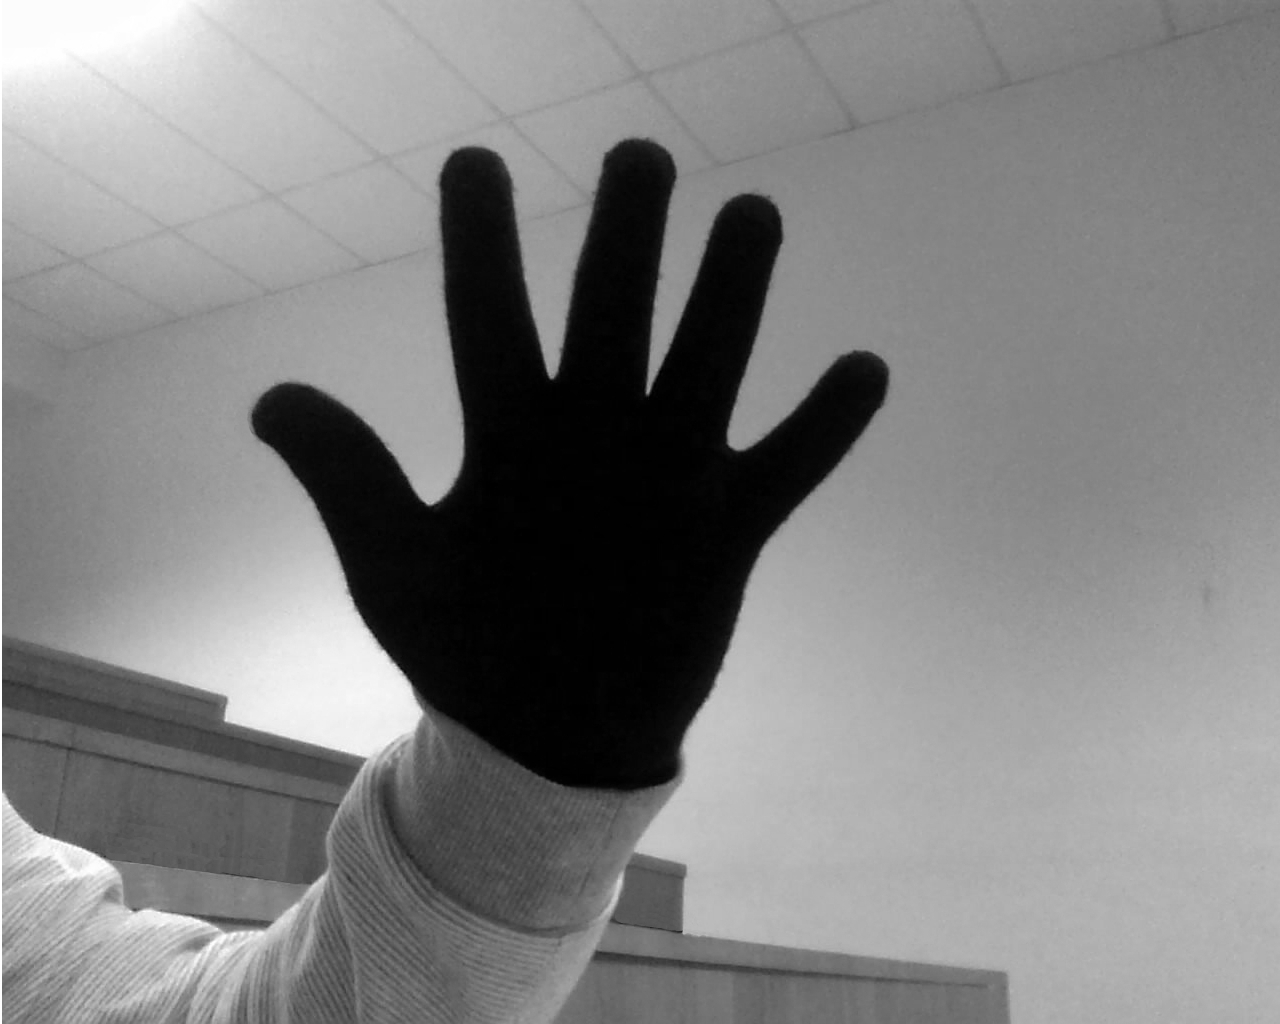
\includegraphics[width=8cm]{sz_base.jpg}
    		\caption{Image capturée en niveaux de gris}
		\end{figure}

    \item Masquage des pixels de la zone couvrant le corps de l'utilisateur. Les pixels de cette zone sont fixés à $255$ (blanc).
    
    \item Binarisation de l'image. Les 1 prennent la place de tous les pixels dont la luminosité est inférieur à $L$.
    
		\begin{figure}[h!]
    		\centering
    		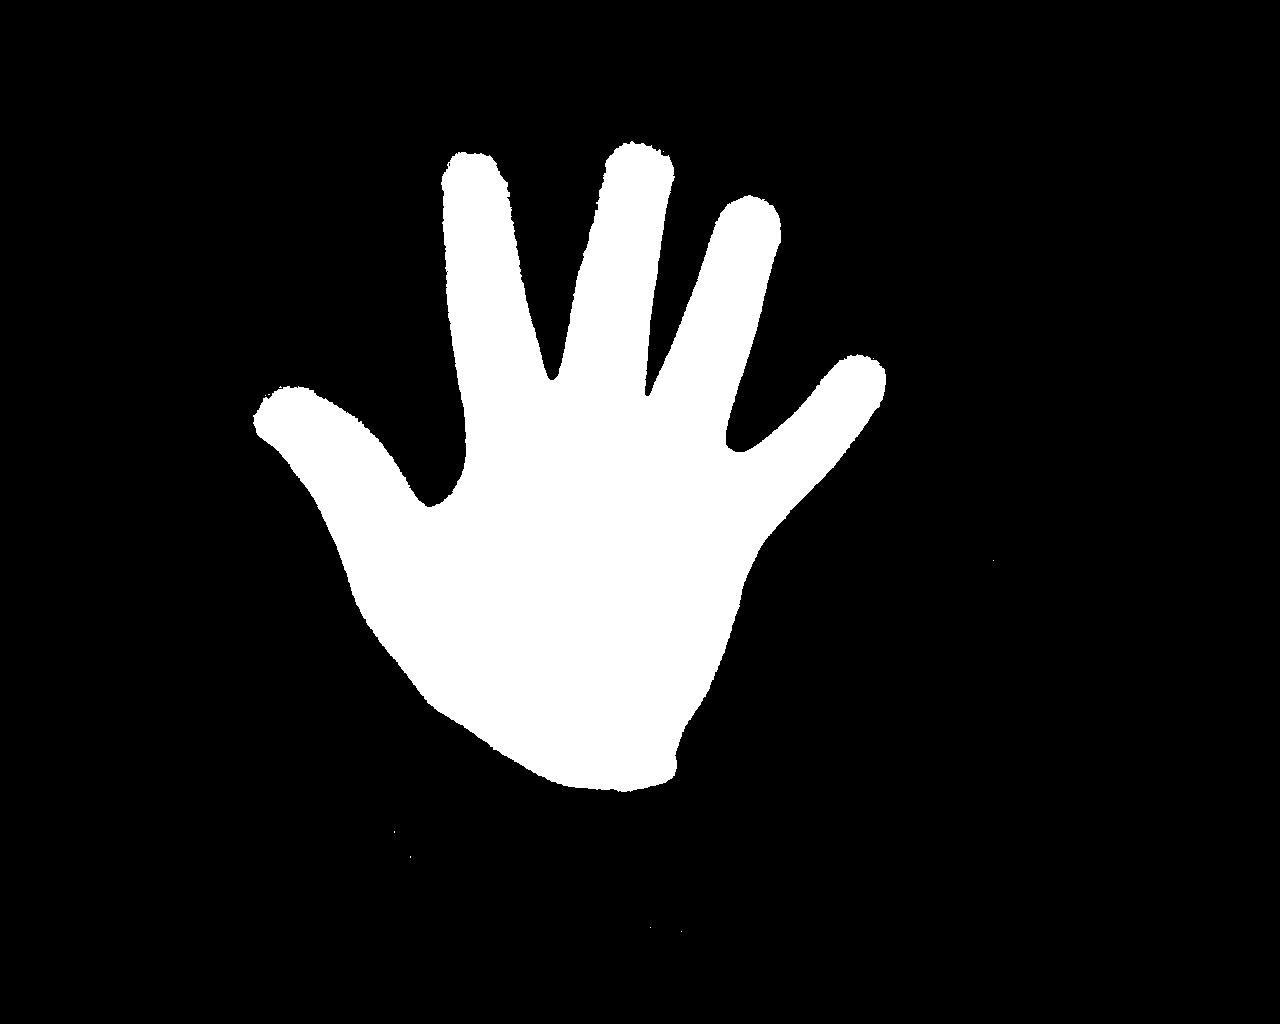
\includegraphics[width=8cm]{sz_bin.jpg}
    		\caption{Image binarisée}
		\end{figure}
    
    \item Érosion de l'image.
	    \par L'érosion est l'une des deux opérations fondamentales du traitement d'image morphologique. Soit A une image binaire et B un élément de structure., l'érosion de A par B est donnée par : $A \bigodot B = \{z|(B)_z \subset A\}$.
    	\par Le résultat de l'érosion ainsi que celui de la dilation n'est pas évident, l'image ne change presque pas. Les différences seront démontrer pendant l'étape de construction de l'enveloppe convexe. 
	    \par Pour l'élément structurant dans l'implémentation nous utilisons une ellipse $3 \times 3$.
	    \begin{table}[h!]
    	    \centering
    	    \begin{tabular}{|c|c|c|}
        	    \hline
        	    0 & 1 & 0 \\ \hline
        	    1 & 1 & 1 \\ \hline
        	    0 & 1 & 0 \\ \hline
        	\end{tabular}
        	\caption{Élément structurant: ellipse $3 \times 3$}
    	\end{table}
    	\par L'érosion est utilisée pour le filtrage du bruit, c'est à dire les  petites particules blanches qui peuvent apparaître sur l'image binarisée par hasard. L'érosion est appliquée à l'image deux fois. Le résultat de l'application est la suppression des petites zones blancs (moins de 4 pixels), les zones correspondant aux mains et seulement elles restent sur l'image. La diminution de leur taille de 2 pixels est compensé pendant l'étape suivante.

    \item Dilatation de l'image.
    	\par La dilatation a pour but de compenser l'utilisation de l'érosion et de  simplifier les frontières des objets. La dilatation est définie comme $A  \bigoplus B = \cup_{b \in B}A_b$. Pour la dilatation le même élément structurant que pour l'érosion dans l'étape précédente. 

    \item La recherche des contours. La recherche des contours est réalisée en utilisant un algorithme basé sur la topologie discrète \footnote{Suzuki, S. and Abe, K., Topological Structural Analysis of Digitized Binary Images by Border Following. CVGIP 30 1, pp 32-46 (1985)}. qui est déjà réalisé dans la bibliothèque OpenCV. La bibliothèque fournit aussi l'algorithme de Teh-Chin \footnote{Teh, C.H. and Chin, R.T.,  On the Detection of Dominant Points on Digital Curve. PAMI 11 8, pp  859-872 (1989)} qui permet diminuer le nombre de points du contour en réunissant les séries des points formant des segments et par cela simplifier les calculs de l'étape suivante.

		\begin{figure}[h!]
    		\centering
    		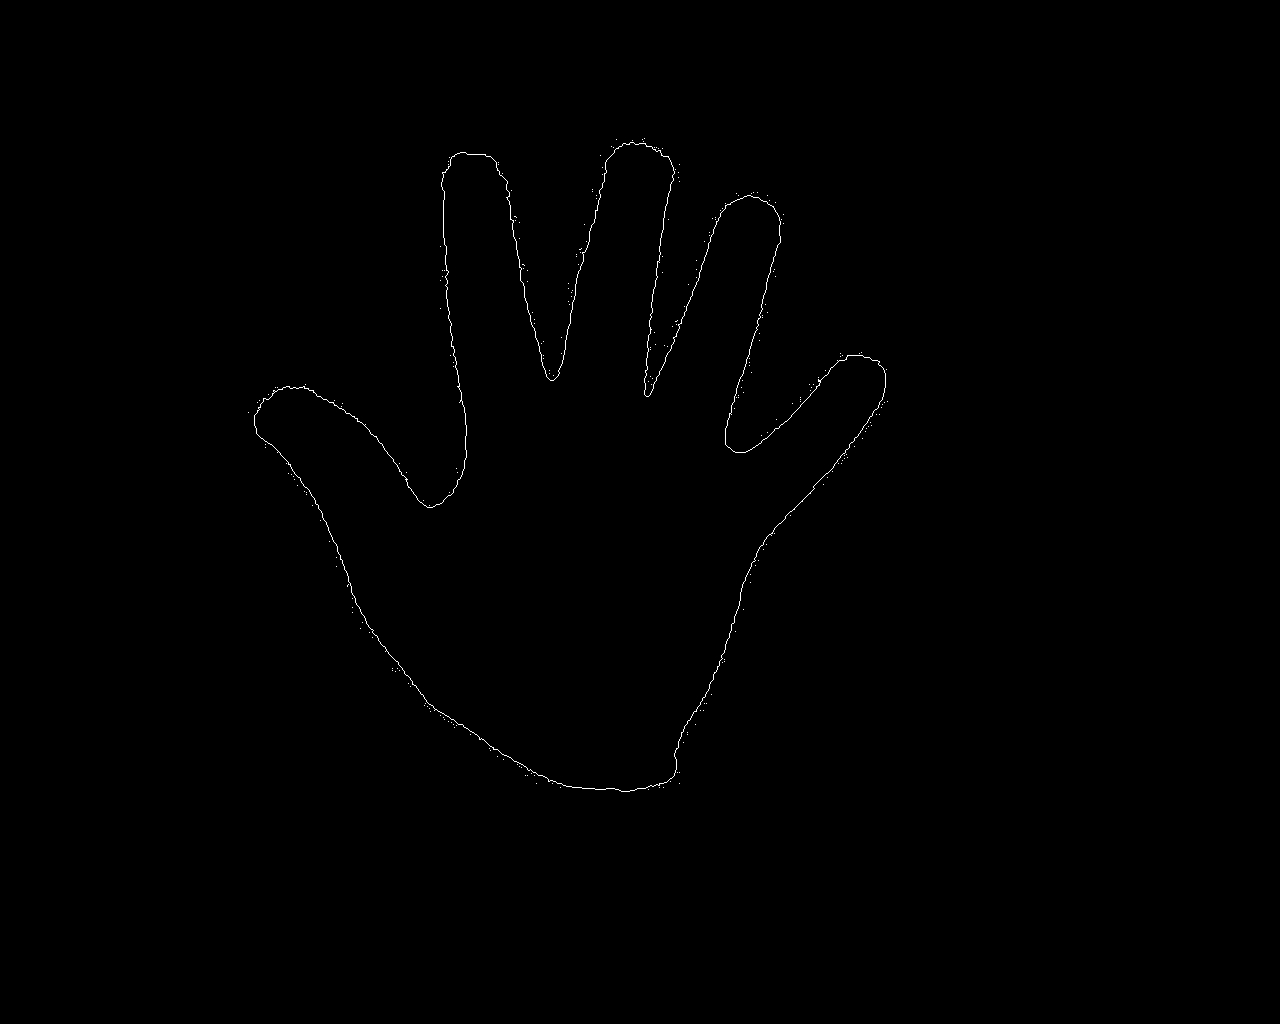
\includegraphics[width=8cm]{sz_contours.jpg}
    		\caption{La détection des contours}
		\end{figure}
    
    \item Construction de l'enveloppe convexe. Les points des contours sont  divisés en deux ensembles selon la partie de l'image (gauche ou droite) à  laquelle ils appartiennent. Pour chaque ensemble on construit une  enveloppe convexe : un polygone convexe tel que tout les points blancs de l'image se situent dedans ce polygone. OpenCV fournit l'algorithme de Sklansky \footnote{Sklansky, J.,  Finding the Convex Hull of a Simple Polygon. pp 79-83 (1982)} qui permet calculer un tel polygone en temps $O(N \cdot log N)$, où $N$ est le nombre de points.
                
		\begin{figure}[h!]
    		\centering
    		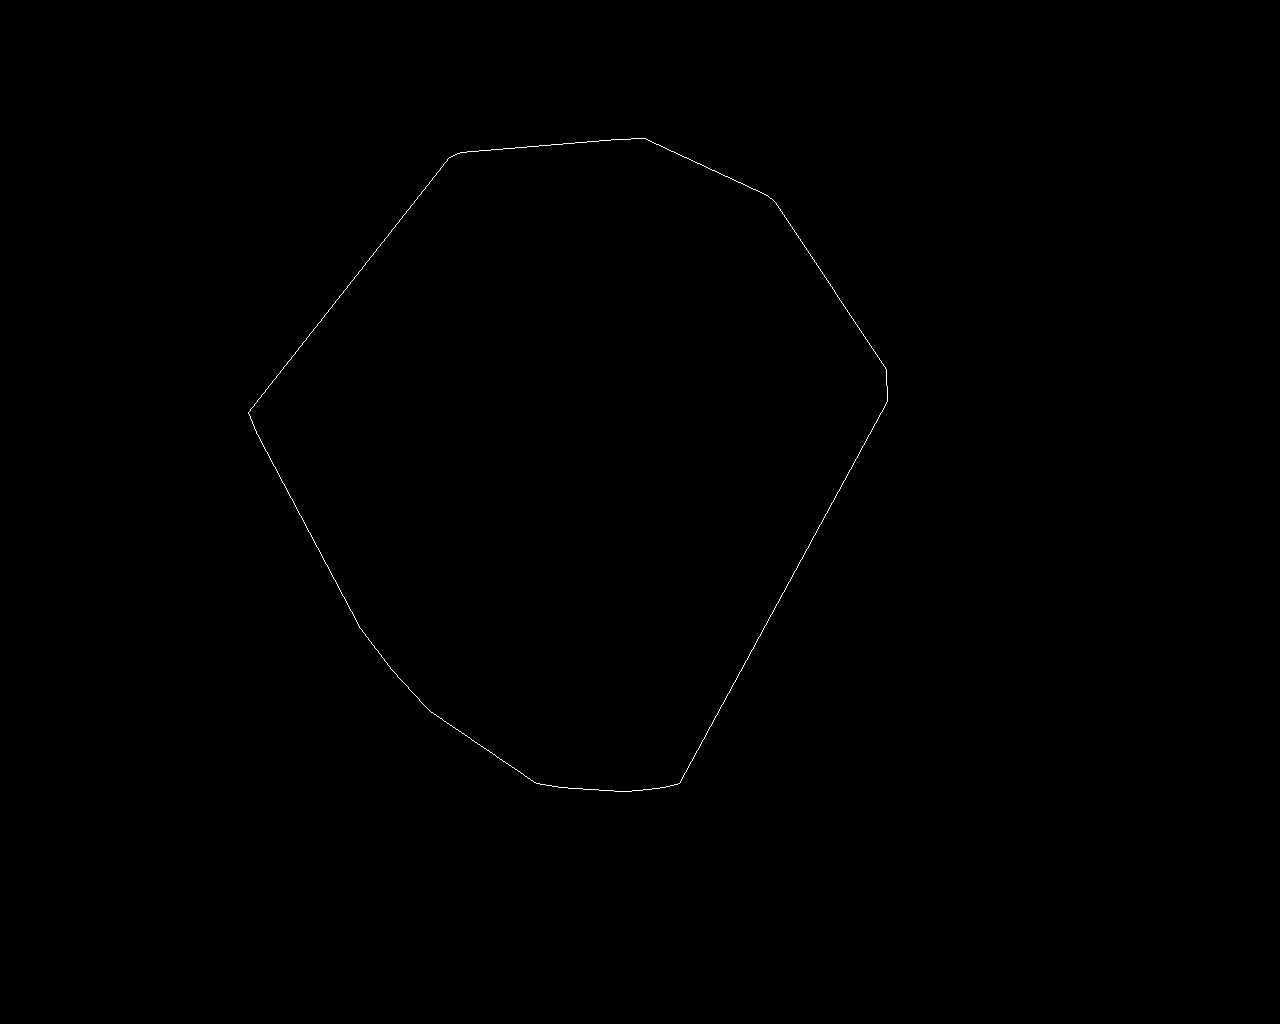
\includegraphics[width=8cm]{sz_hull.jpg}
    		\caption{Enveloppe convexe}
		\end{figure}

		\par Montrons le résultat de la construction de l'enveloppe convexe pour l'image à laquelle on n'a pas appliqué l'étape d'érosion/dilation. La figure~\ref{erosion} montre l'enveloppe construite à partir de l'image initiale sans application de ces deux étapes.

		\begin{figure}[h!]
		    \centering
		    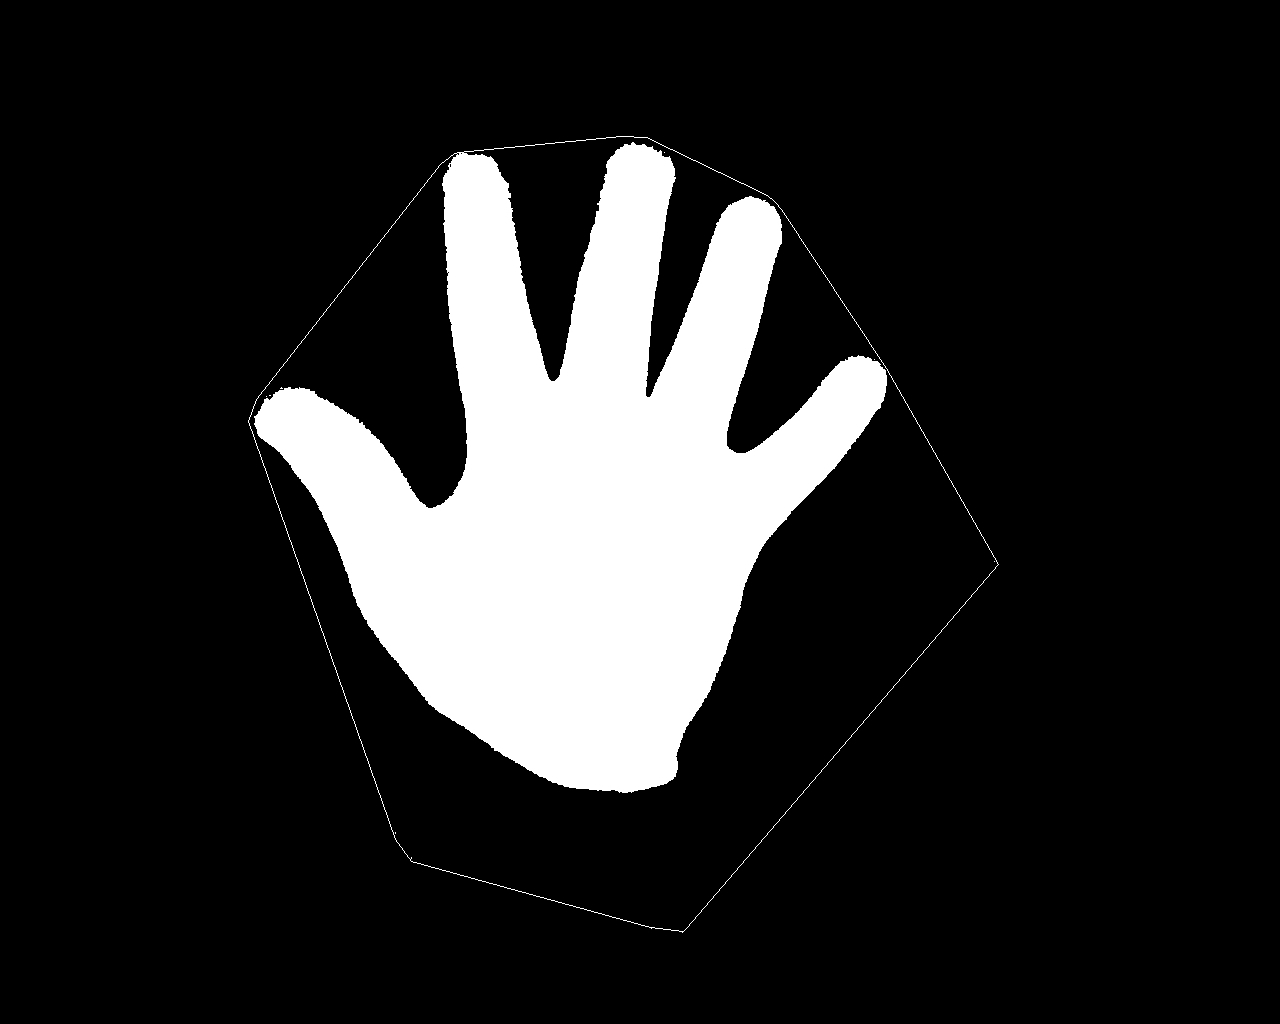
\includegraphics[width=8cm]{sz_bad_hull.jpg}
		    \caption{Démonstration de la raison d'application de l'érosion/dilation}
		    \label{erosion}
		\end{figure}

    \item La moyenne des coordonnées de chaque enveloppe est considérée comme la  coordonnée de la main. La surface du polygone qui est facile à calculer (somme des surfaces des triangles) est comparé avec la valeur du seuil de la surface calculée lors de la calibration. Si la surface dépasse le seuil, la main est considerée ouverte, sinon on la considère comme fermée. En gardant la position précedente des mains on peut calculer la vitesse. En disposant de la vitesse courante et de celle de l'étape précedente on calcule l'accélération. On n'a donc besoin que de l'image courante ainsi que de la vitesse et la position à l'étape précédents pour calculer toutes les caractéristiques des mains. On les transmet alors au module de gestion des événements.

    \item On recommence la boucle.
\end{itemize}

\section{Caractérisation des évènements}
\subsection{Introduction}
\par La caractérisation des évènements correspond à l'interprétation des gestes de l'utilisateur à travers différentes zones décrites par ce dernier et au déclenchement de signaux MIDI associés. Pour chaque zone, on a pu associer un évènement à un signal MIDI. Visuellement, lorsqu'un évènement est détecté dans une zone, celle-ci est mise en valeur dans l'affichage. En entrée, on dispose de positions des mains et de leurs ouvertures. En sortie, on appelle des fonctions d'envoi de signaux MIDI.
\subsection{Description des zones}
\par  Une zone est décrite initialement par sa position, sa taille, son type  (fader, pad ou segment) et, pour chaque événement, un ensemble de  signaux MIDI (éventuellement vide) qui doivent être déclenché lorsque cette événement est détecté.
\par  Pour détecter un événement, on dispose de l'historique des positions et vitesses de chaque main. On s'intéresse aux deux dernières entrées de l'historique et de l'état de la main, ouverte ou fermée. De ces informations on détecte directement l'entrée/sortie d'une zone et le franchissement d'un segment. La bibliothèque Qt fournit en effet des fonctions qui permettent de savoir si un point est dans un rectangle et si deux segments se coupent.
\par Le franchissement d'un segment est orienté. Le sens est déterminé par signe du déterminant lors du calcul d'intersection entre le segment et et le segment formé par les deux dernières positions de la main. 
\par La frappe est détéctée lors d'un changement de du sens de la vitesse et lorsque la norme des vitesses atteint une certaine valeur. On calcule en fait l'accélération. Malheureusement, le choix de la valeur seuil est expérimentale et n'a pas donné de résultat suffisamment stable pour être utilisable.
\par Pour les autres événements, il nous faut  également l'état de la zone :
\begin{itemize}
    \item active ou non pour lancer ou arrêter un clip
    \item l'ouverture de la main à l'entrée dans la zone pour les faders,  une main qui rentre fermée dans un fader ne doit pas changer sa valeur. Une fois l'utilisateur saisi du curseur, s'il reste immobile, la position calculée peut varier sensiblement. Pour que la valeur du fader ne joue pas au yoyo, on s'assure que la position de la main ait varié suffisamment pour répercuter le changement sur la valeur du fader.
\end{itemize}
\subsection{Implémentation}
\par  La détection et le déclenchement de signaux sont réalisés par les  zones. La gestion des événements consiste à envoyer à chaque  zone ou segment les informations suffisantes relatives à la main. Il s'agit  donc d'une boucle disposant de la liste des zones (fournis par la  configuration) qui la parcourt en appelant pour chaque zone la  détection.
\par Chaque zone disposant d'une table de correspondance entre évènements et signaux, on envoie les signaux MIDI associées aux évènements détéctés. Pour les faders et pad XY, on modifie un des octets du signal MIDI pour faire la correspondance avec le niveau du curseur avant l'envoi.
\subsection{Affichage des zones}
\par  Les zones et les segments sont dessinés sur un Label Qt qui est superposé à l'image de la caméra avec de la transparence. Les segments sont orientés par une fléche. Il s'agit également de montrer quelles zones sont actives et donc d'offrir un support visuel à l'utilisateur. Celui-ci peut ainsi savoir où se trouve les zones par rapport à lui et controler leur activation.
\section{Interface MIDI}
\par MDMA est un contrôleur MIDI virtuel : il communique avec des logiciels/appareils musicaux au moyen de signaux MIDI. On l'utilisera par exemple en le connectant à un séquenceur, c'est-à-dire un programme permettant l'enregistrement et l'arrangement de mutliples pistes, ou bien à un sampler\footnote{outil permettant de rejouer des échantillons sonores préalablements enregistrés} ou un logiciel de DJing\footnote{logiciel utilisé par les DJ en remplacement ou complément des platines traditionnelles} (voir figure~\ref{logiciels}).
\begin{figure}
    \centering
    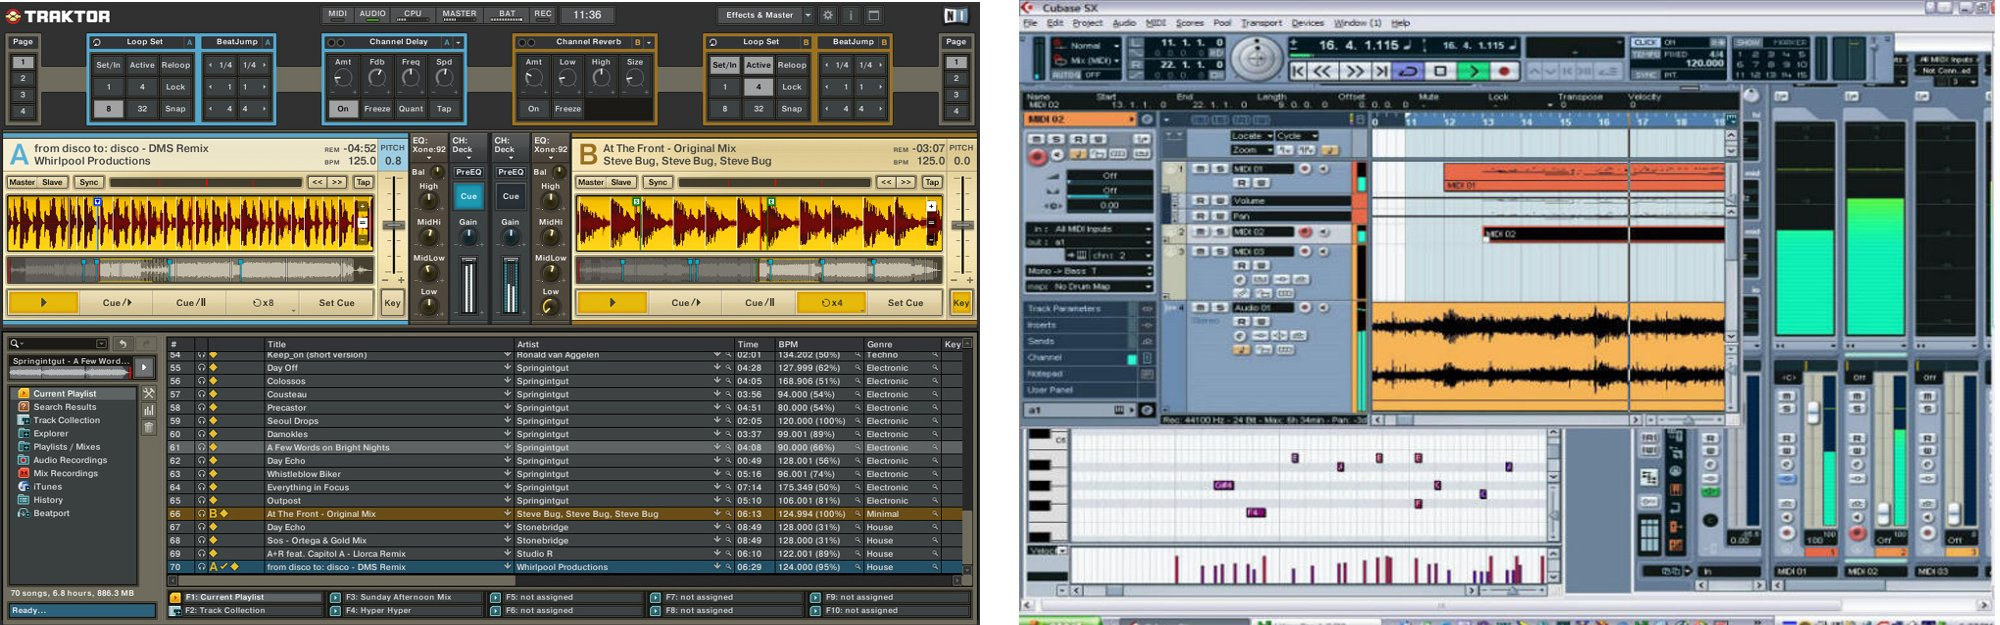
\includegraphics[width=12cm]{logiciels.jpg}
    \caption{Quelques logiciels de musique assistée par ordinateur}
    \label{logiciels}
\end{figure}
\par La norme MIDI a été créée dans les années 80 pour permettre la communication entre divers appareils de musique électronique, notamment pour transférer des notes ou les paramètres des synthétiseurs. Aujourd'hui, elle est encore utilisée et la plupart des logiciels musicaux actuels peuvent être commandés par des signaux MIDI.
\par On peut ainsi modifier en direct des paramètres divers comme le volume sonore, la hauteur d'une note, ou bien lancer des commandes destinées à lire une boucle, jouer des notes particulières sur un synthétiseur... Ces commandes sont entièrement assignables et configurables par l'utilisateur. L'adoption de la norme MIDI par de très nombreux constructeurs et éditeurs du monde de la musique garantit la polyvalence de notre programme.
\par Un message MIDI est toujours composé d'un octet de statut suivi de plusieurs octets de données (voir figure~\ref{note_on}) :
\begin{itemize}
    \item l'octet de statut commence par un 1, suivi de trois bits  déterminant le type de message (il y a huit types possibles, appelés  "note off", "note on", "polyfonic aftertouch", "channel pressure",  "program change", "control change", "pitch bending" et "system", bien  que certains, comme "polyfonic aftertouch", soient beaucoup plus  rarement utilisés que d’autres), de quatre bits déterminant le canal du  message (un appareil ou un logiciel peut être configuré pour n’écouter  que certains canaux)
    \item les octets de données commencent par un 0, suivi de 7 bits codant la valeur de la donnée (la note jouée pour la première donnée d'un note on, et sa vélocité pour la seconde)
\end{itemize}
\begin{figure}
    \centering
    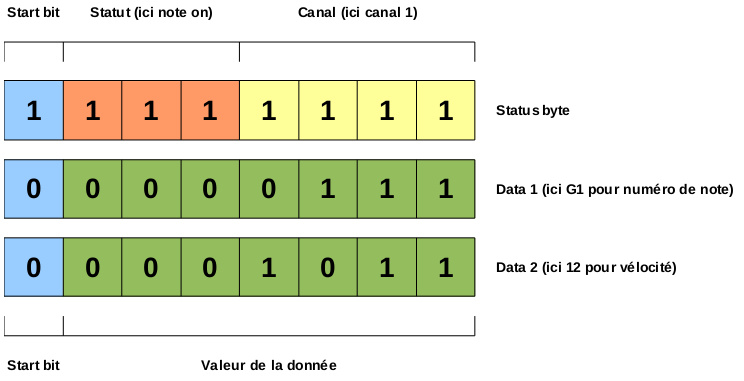
\includegraphics[width=12cm]{note_on.jpg}
    \caption{La structure d'un message MIDI de type note on}
    \label{note_on}
\end{figure}
\par Pour gérer toutes les tâches concernant le protocole MIDI, nous avons décidé d'utiliser la bibliothèque RtMidi. Toujours développée, cette bilbiothèque orientée programmation objet pour le C++ est multi-platforme (Linux, Windows et Mac OS). Nous exploitons essentiellement la classe RtMidiOut, qui gère l'envoi de messages MIDI en temps réel.
\par La première chose à faire est d’ouvrir un port MIDI virtuel pour y envoyer nos messages. Sous systèmes Linux et Mac cette opération est directement prise en charge par RtMidi, et un élément externe peut écouter les messages MIDI envoyés par MDMA sur le port qu'il a créé (figure~\ref{MDMA_port}); sous Windows ce n’est pas le cas\footnote{il n'est malheureusement pas précisé pourquoi} et nous utilisons alors un driver MIDI virtuel tel que loopMIDI\footnote{http://www.tobias-erichsen.de/software/loopmidi.html} ou LoopBe1\footnote{http://nerds.de/en/loopbe1.html} pour contourner ce problème : ces logiciels permettent de créer deux ports MIDI, un d’entrée et un de sortie, et font transiter tout message reçu par le port d’entrée vers le port de sortie. MDMA n’a donc qu’à envoyer ses messages sur le port d’entrée, ceux-ci pourront être  récupérés par n’importe quel logiciel écoutant sur le port de sortie (figure~\ref{External_port}).
\begin{figure}[h]
    \centering
    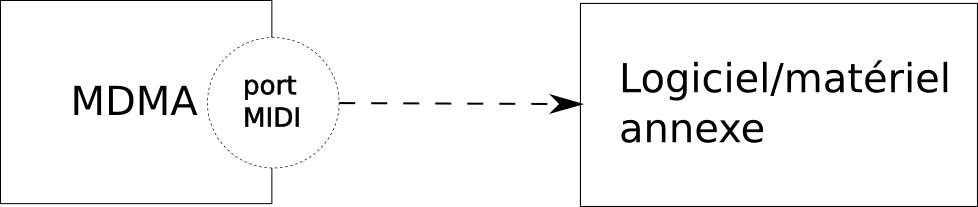
\includegraphics[width=12cm]{midi.png}
    \caption{Sous Linux et OS X, MDMA est capable de créer un port MIDI sur lequel des éléments externes peuvent écouter les messages qu'il envoie}
    \label{MDMA_port}
\end{figure}
\begin{figure}[h]
    \centering
    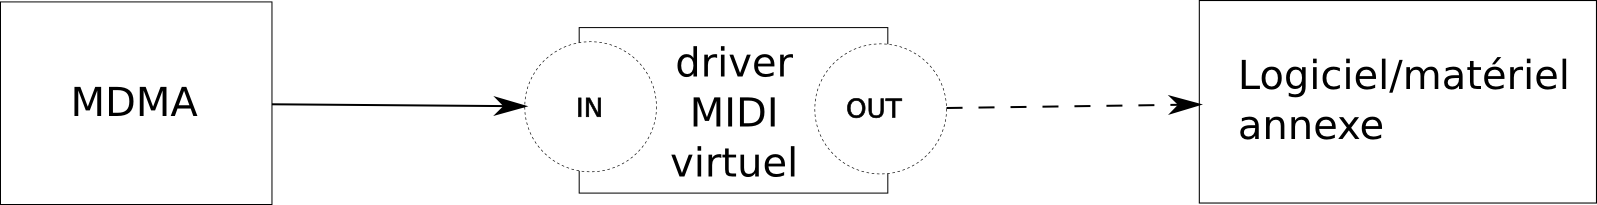
\includegraphics[width=12cm]{midi2.png}
    \caption{L'utilisation d'un driver MIDI virtuel exterieur permet de se passer de la création d'un port MIDI : MDMA se connecte à l'entrée et les éléments externes peuvent écouter les messages qu'il envoie se connectant à la sortie}
    \label{External_port}
\end{figure}
\par Une fois la manière de procéder déterminée (création ou non d'un port directement par MDMA), la gestion des messages est très simple : RtMidiOut possède une méthode \emph{sendMessage} permettant d'envoyer un \emph{std::vector<unsigned char>} (représentant un message MIDI) sur le port précédemment choisi.
\par L'envoi de messages est commandé par les mouvements de l'utilisateur, et s'effectue en bout de chaîne de la gestion des événements.
\section{Compilation et installation}
\par Les adeptes de musique assistée par ordinateur travaillent souvent sous Windows ou Mac OS, il était donc capital de fournir une version fontionnelle de MDMA pour chacun de ces systèmes. Il fallait également garder à l'esprit que le musicien lambda est peu habitué à compiler les sources d'un programme. Nous avons dû rendre la procédure d'intallation de MDMA la plus simple d'accès possible. Les sources du logiciel ainsi que les différents exécutables mentionnés dans cette section sont disponibles au téléchargement sur le site Internet du projet (\url{http://graal.ens-lyon.fr/mdma}).
\subsection{Linux}
\par Contrairement aux utilisateurs utilisation des systèmes Windows et Mac, les utilisateurs de Linux sont généralement demandeurs de sources pour tous les projets libres. L'utilisation de gestionnaire de paquets ainsi que de l'assistant à la compilation (\texttt{Make} et affiliés) permet par ailleurs de faciliter grandement toute la procédure de compilation.
\par Nous avons donc choisi de proposer le projet sous forme d'une archive contenant (entre autres) :
\begin{itemize}
    \item Les sources
    \item Un fichier de projet (\texttt{.pro}), permettant de générer un \texttt{Makefile} a l'aide de \texttt{qmake}
    \item Un script bash écrit par nos soins, vérifiant les dépendances vis-a-vis des librairies externes libres et demandant a l'utilisateur d'installer les librairies manquantes le cas échéant
\end{itemize}
\subsection{Windows}
\par La compilation sous système Windows étant relativement fastidieuse, nous avons décidé de proposer à l'utilisateur un installateur pour MDMA. Pour ce faire, nous avons compilé une version exécutable du logiciel avant de l'insérer avec les bibliothèques requises dans un installateur à l'aide du logiciel InstallForge\footnote{InstallForge : \url{http://installforge.net/}}. Cela permet par ailleurs de s'assurer de l'installation des dépendances \texttt{.dll} au bon endroit (même dossier que l'exécutable).
\subsection{Mac OS}
\par Cet étape nous a posé quelques soucis : du fait de restrictions sur les licences libres, Mac OS ne dispose pas d'une version récente de GCC, il a donc fallu adapter tout le code source pour se passer des spécifications C++11. Nous avons ensuite pu construire un binaire exécutable incluant toutes les dépendances (bibliothèques graphiques, MIDI…).
\section{Communication}
\subsection{Introduction}
\par L'équipe chargée de la communique s'occupe de la communication du projet sur deux échelles, en externe et en interne. La communication externe concerne l'ensemble des liens entre \emph{MDMA} et les acteurs extérieurs (que ce soit par voie numérique -- site Web, courriels -- ou par voie orale). La communication interne consiste à gérer les discussions dans l'équipe, ainsi qu'avec les responsables du projet et du département.
\subsection{Définition d'une identité graphique}
\par Pour débuter une bonne communication, il faut d'abord réfléchir à l'image que l'on veut donner au projet. MDMA a pour but de développer un logiciel innovant : l'interface homme-machine se veut délibérément moderne, sans clavier ni souris l'utilisateur peut commander son ordinateur pour produire des signaux musicaux. Mais il s'inscrit dans une tendance alternative, celle de la musique électronique et des synthétiseurs sonores. Nous avons cherché à construire une identité assez \emph{rétro} mais véhiculant la nouveauté du projet.
\par Nous sommes parti d'un ensemble de couleurs très vivantes -- du jaune au rouge -- assez agressives :
\begin{figure}[h]
  \centering
  
\includegraphics[width=10cm]{comm-swatch.pdf}
  \caption{Gamme de couleurs utilisées pour la charte graphique}
  \label{fig:swatch}
\end{figure}
\par Avec ces couleurs, nous avons pu réfléchir à un logotype. Plusieurs pistes étant possible, celle d'un texte uniquement (« MDMA ») assez minimaliste a été privilégié, avec une police très \emph{pixelisée}. Trois propositions ont été réalisées pour affiner le logo :
\begin{figure}[h]
  \centering
    
\includegraphics[width=8cm]{comm-logos.pdf}
  \caption{Trois propositions de logotype}
  \label{fig:Logos-MDMA}
\end{figure}
\par Le premier graphique a été sélectionné par l'équipe, et rapidement intégré au site Internet.
\subsection{Communication externe}
\paragraph{Internet}
\par Afin d'obtenir un minimum de visibilité, le projet avait besoin d'une présence sur Internet. Nous avons donc d'abord travaillé à mettre en place un site Web. Nous avons conçu une interface assez minimaliste, fondée sur les couleurs de la gamme représentée à la figure~\ref{fig:swatch}.
\par Le site Internet (\url{http://graal.ens-lyon.fr/mdma/}) contient différentes informations, dont :
\begin{itemize}
  \item une présentation du projet, minimale sur la première page, puis détaillée par la suite ;
  \item les nouveautés au fil du projet ;
  \item les liens pour télécharger le logiciel et des aides pour le compiler si nécessaire ;
  \item une description complète de chaque \emph{workpackage} ainsi que leurs avancées et découvertes au fil du temps ;
  \item une page personnelle pour chaque membre, avec la possibilité de nous contacter.
\end{itemize}
\par Le site est fondé sur \emph{Wordpress} -- un moteur dynamique -- qui nous permet de gérer des commentaires pour chaque page, une première page dynamique avec la liste des derniers articles, des flux RSS… Par ailleurs, un \textbf{travail de traduction} a été réalisé sur presque l'intégralité du site, pour obtenir un site entièrement trilingue, en français, en anglais et en russe : les 23 pages du sites sont traduites dans ces trois langues. Un menu en haut du site contient des boutons avec icônes pour sélectionner la langue ; par ailleurs, selon la langue du navigateur, la langue optimale pour l'utilisateur est automatiquement choisie.
\begin{figure}[p]
  \centering
    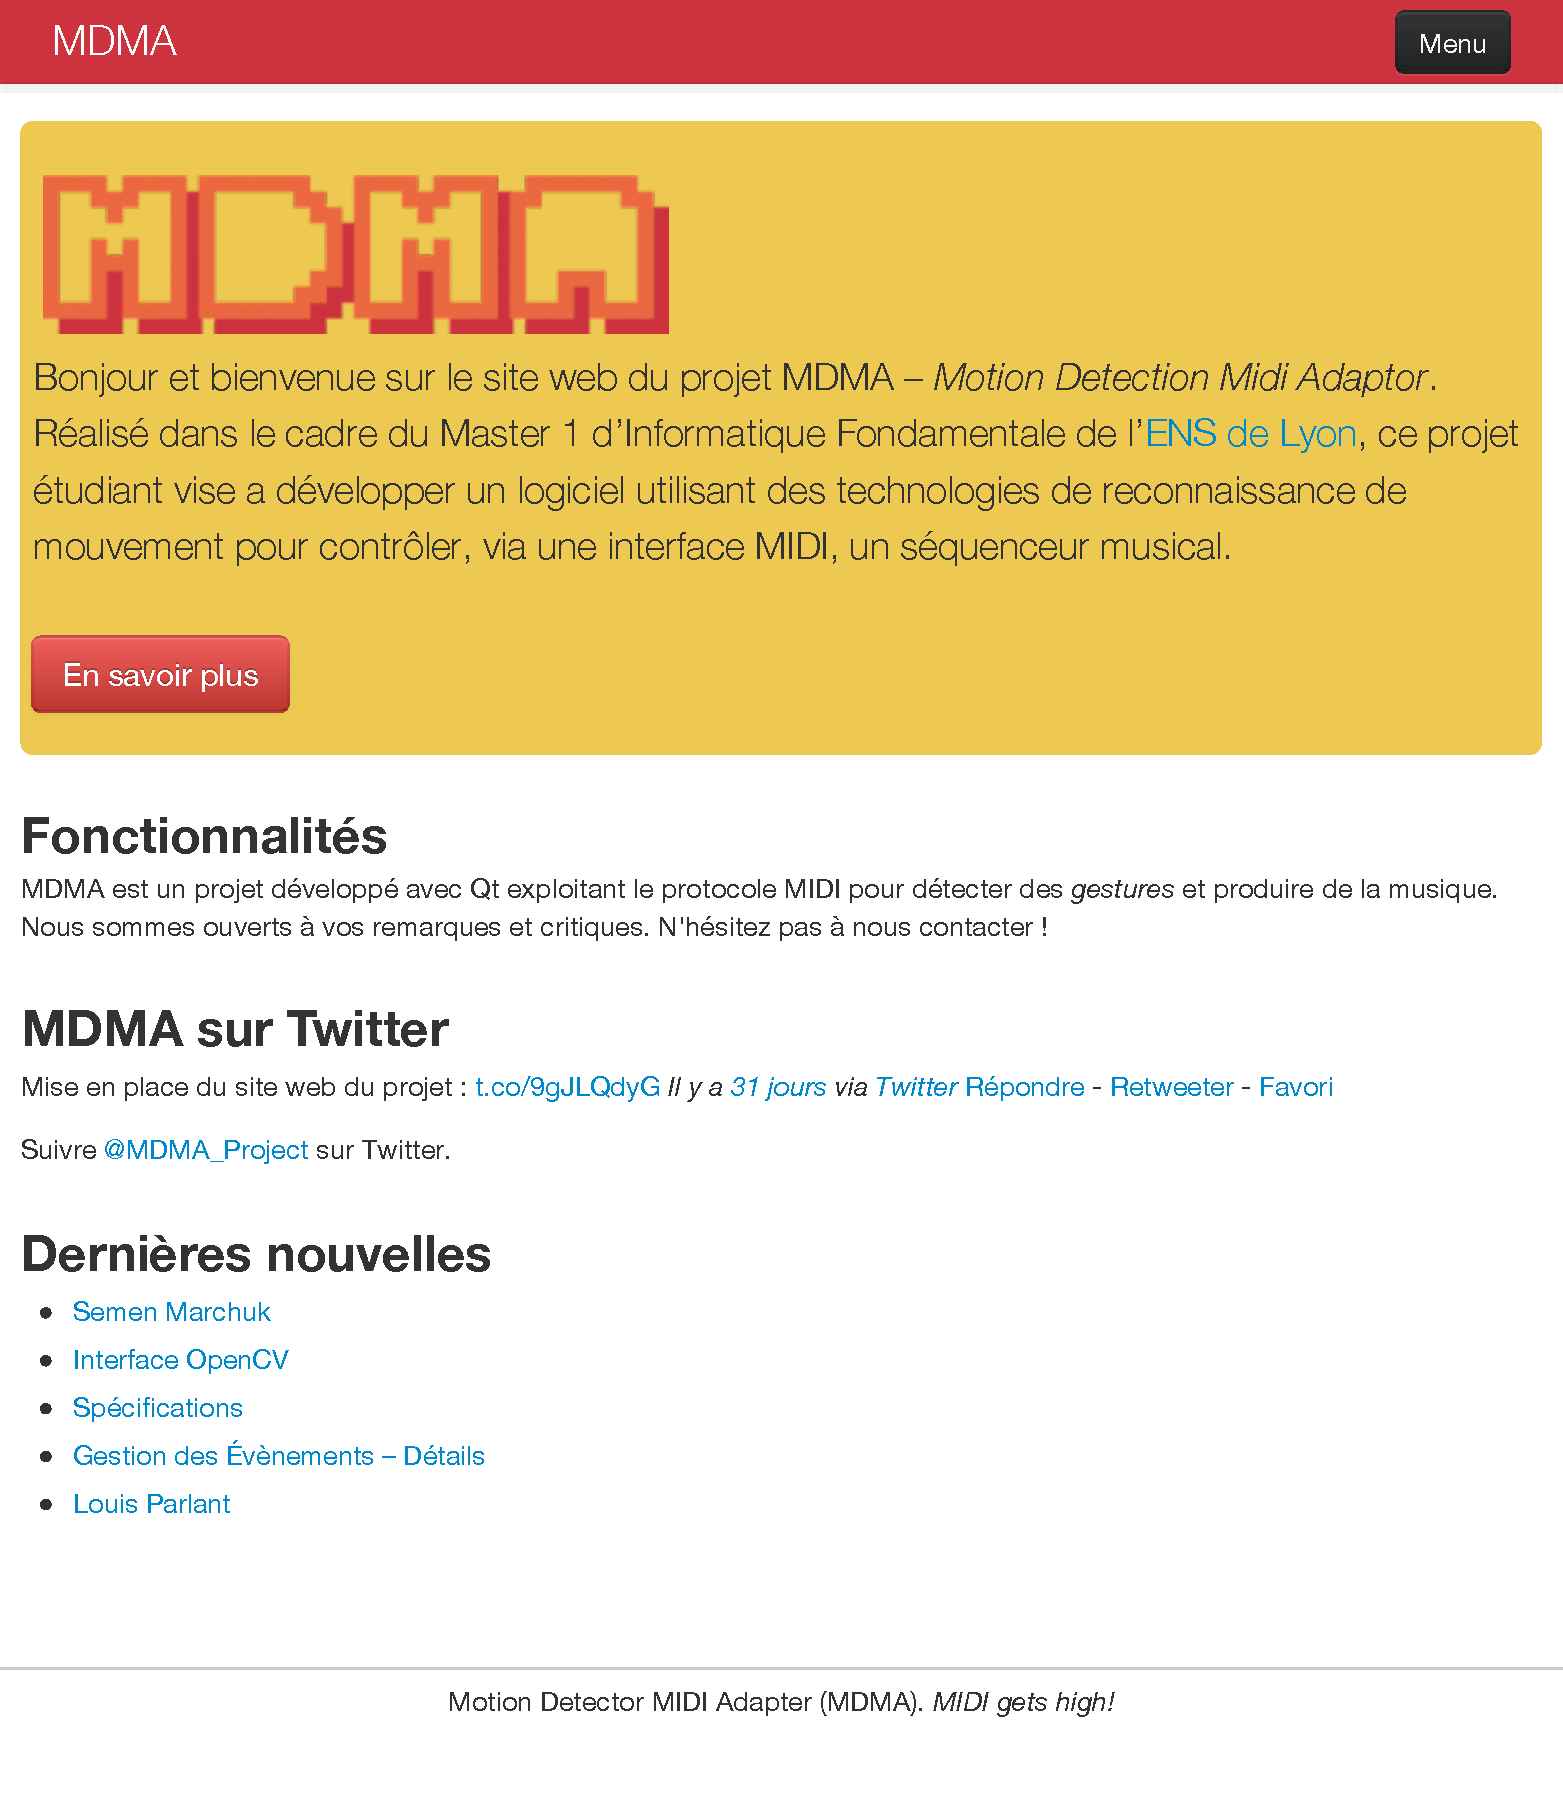
\includegraphics[width=8cm]{comm-web2.pdf}
  \caption{Capture d'écran du site (version mobile)}
\end{figure}
\begin{figure}[p]
  \centering
    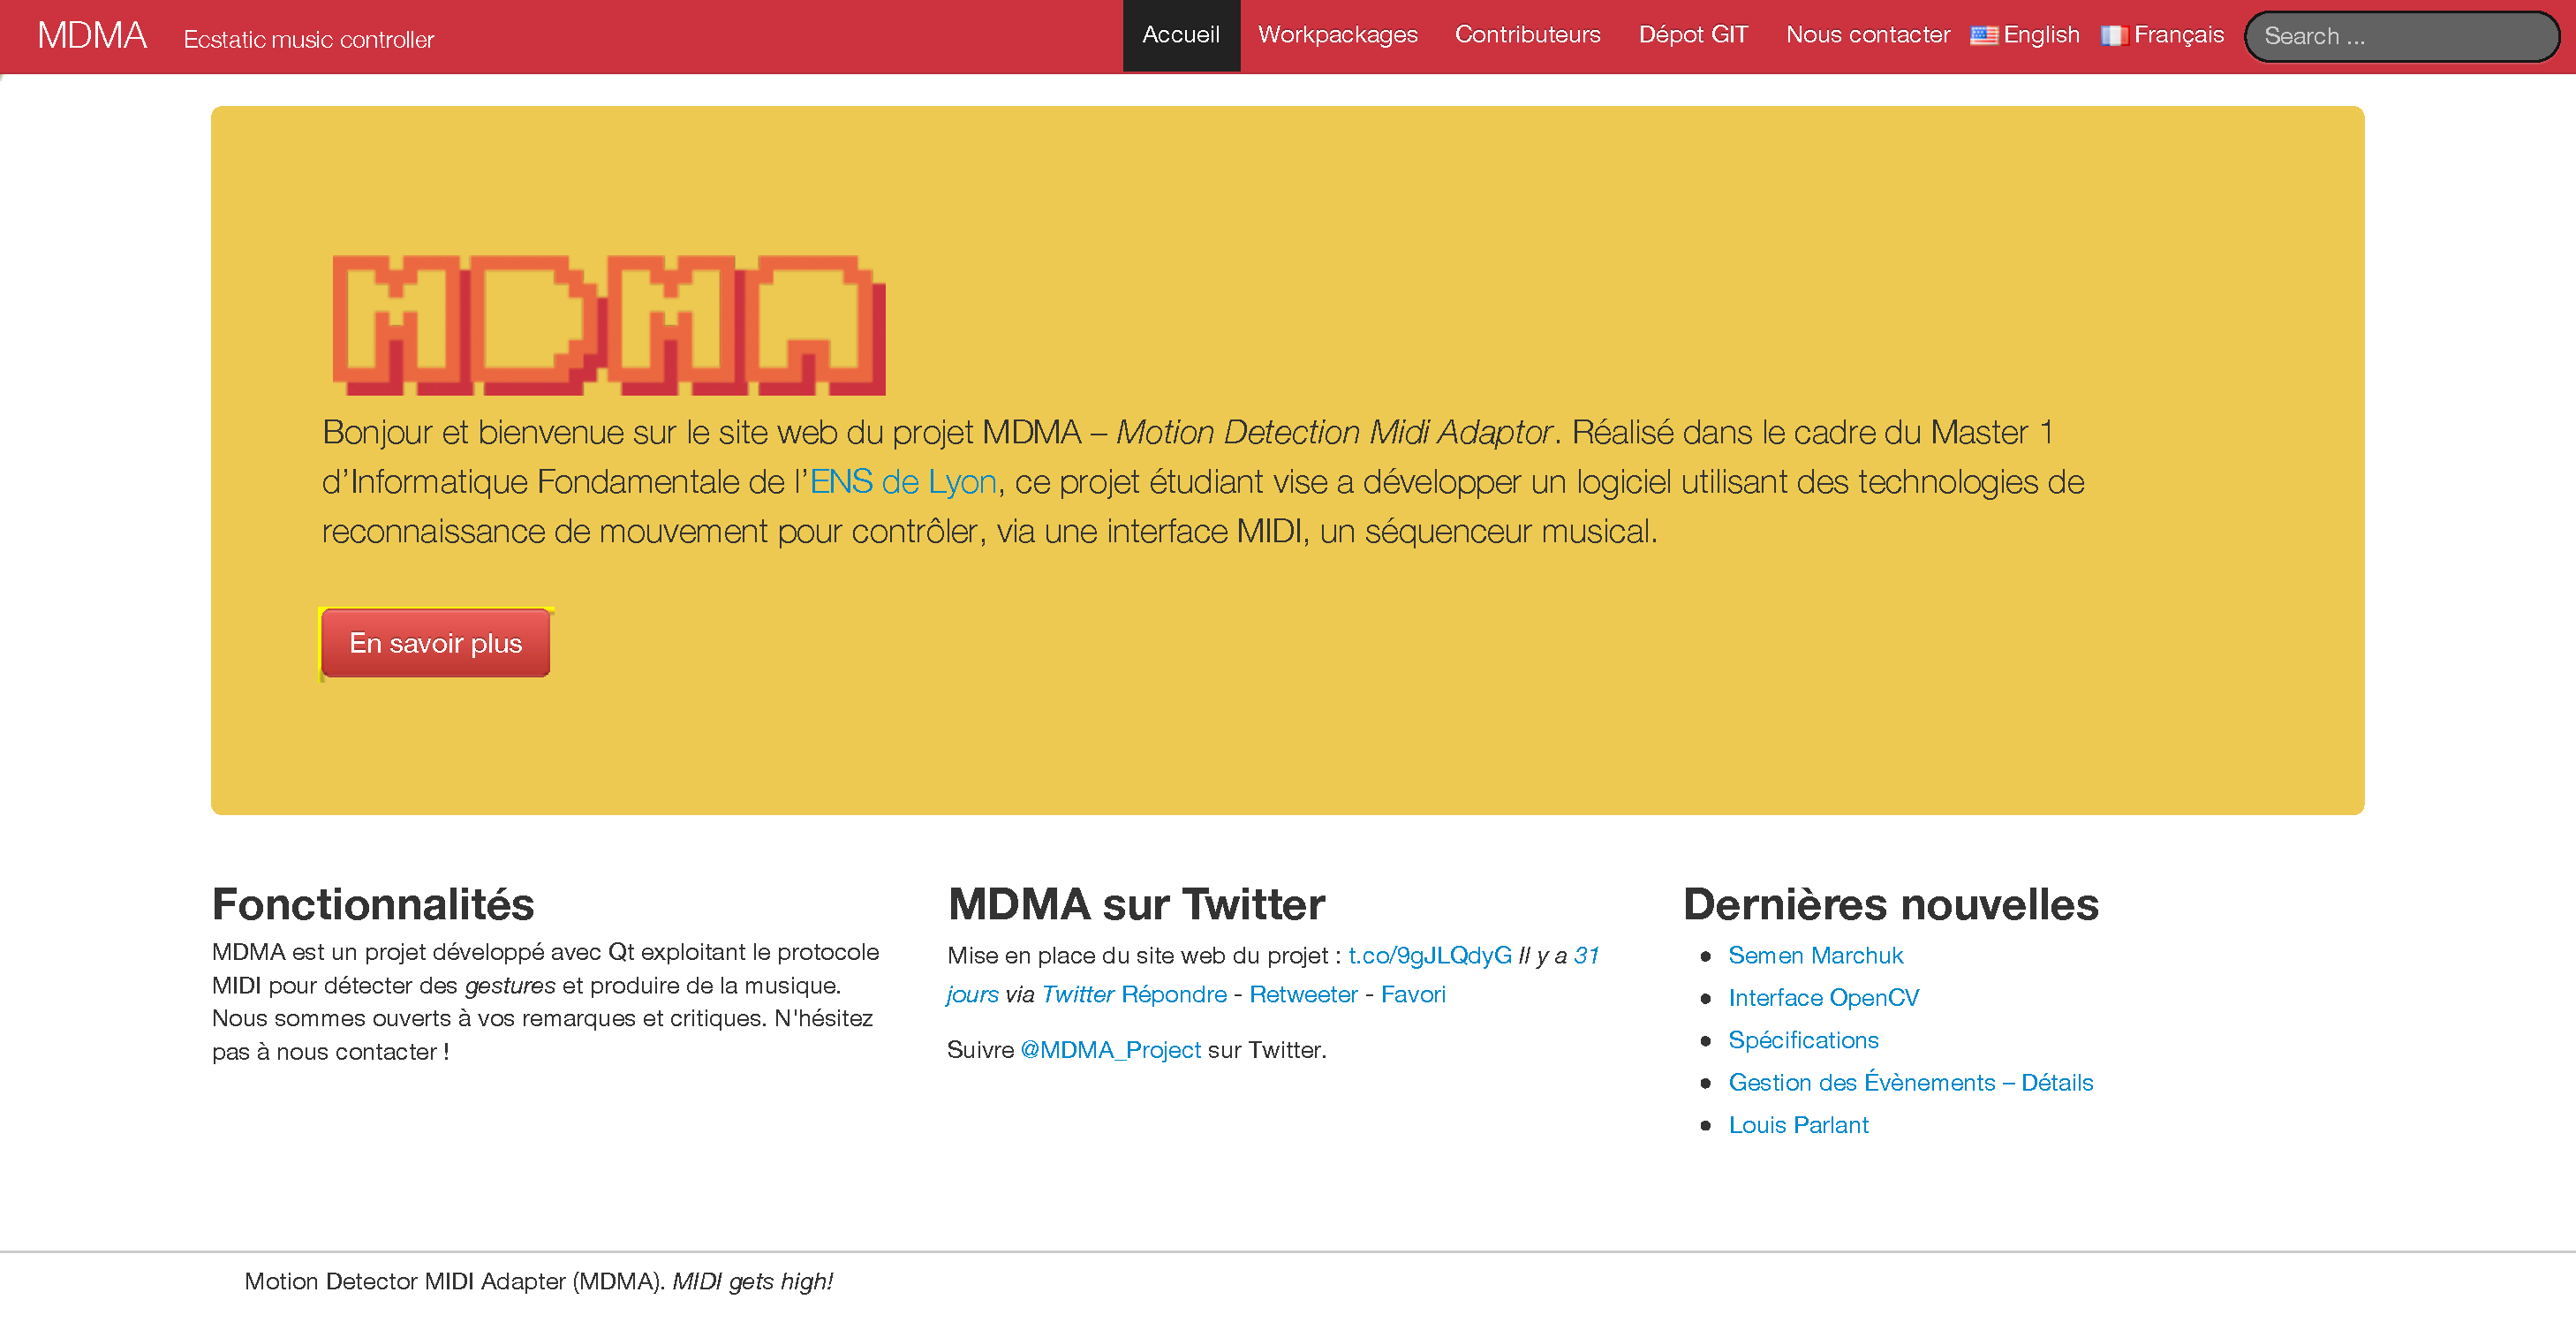
\includegraphics[width=10cm]{comm-web1.pdf}
  \caption{Capture d'écran du site du projet}
\end{figure}
\paragraph{Diffusion dans l'école}
\par Le projet dispose aussi d'un page sur \emph{Facebook} (\url{http://www.facebook.com/mdma.project}). Associé à des communications dans l'école (journal des étudiants, affiches), nous avons pu aller au devant des étudiants pour leur montrer notre projet, les faire participer aux rendez-vous et essais du logiciel.
\subsection{Autres présences}
\par L'équipe « communication » se charge du lien entre le projet et l'équipe pédagogique, par exemple pour des questions de budget (le financement l'année dernière d'un \emph{Microsoft Kinect} par exemple) ; il a aussi pour vocation de diffuser notre projet à des musiciens et des personnes intéressées par la musique électronique. Nous avons ainsi cherché des utilisateurs capable de tester MDMA et de produire des retours en situation réelle. Depuis la finalisation du logiciel, nous avons pu recontacter plusieurs spécialistes (producteurs, DJs) motivés qui souhaitaient diffuser MDMA au sein de leurs équipes. Nous sommes prêts à les suivre dans les semaines qui suivent afin de concrétiser ce logiciel avec des essais grandeur nature, dans des espaces de concerts par exemple.
\section{Une utilisation concrète de MDMA}
\par Voici un exemple d'utilisation de MDMA avec le logiciel \emph{Ableton Live}, particulièrement adapté au contrôle MIDI.
\par Il faut avant tout calibrer MDMA. Une fois cette étape effectuée, il faut configurer les communications MIDI en choisissant un port auquel on connectera \emph{Live}. On peut ensuite créer les zones dont on aura besoin et ainsi fabriquer de toutes pièces sa surface de contrôle.
\par Pour chaque zone, il faut définir les messages MIDI à envoyer et en préciser les paramètres qui dépendent des coordonnées de la main de l'utilisateur le cas échéant. L'interprétation d'un message dépend de son numéro de commande et de son canal : il faut donc faire attention à donner des numéros ou des canaux différents à des messages que l'on souhaite faire correspondre à des ordres de types différents. En pratique, on peut utiliser les différents canaux pour classer les messages que l'on envoie.
\par Pour mettre en place la communication MIDI avec le logiciel qu'on veut contrôler, il faut d'abord connecter ce logiciel au même port MIDI que MDMA. Par exemple, dans \emph{Live}, il faut identifier notre port MIDI comme surface de contrôle, et éventuellement comme entrée MIDI sur les pistes où l'on veut envoyer des notes.
\par Il faut ensuite réaliser les différentes assignations des commandes. La majorité des logiciels de musique disposent d'une fonction \emph{MIDI learn}. Celle-ci permet au logiciel de reconnaître les identifiants du message qu'on lui envoie et de l'associer à une action précise. Il nous suffit donc de choisir l'action à déclencher, et, dans MDMA, de réaliser l'événement censé la contrôler. Une fois que toutes les zones sont assignées à des actions du logiciel (on parle de \emph{mapping}), MDMA est complètement associé au logiciel et peut le contrôler (voir figure ~\ref{live}).
\begin{figure}[h]
  \centering
    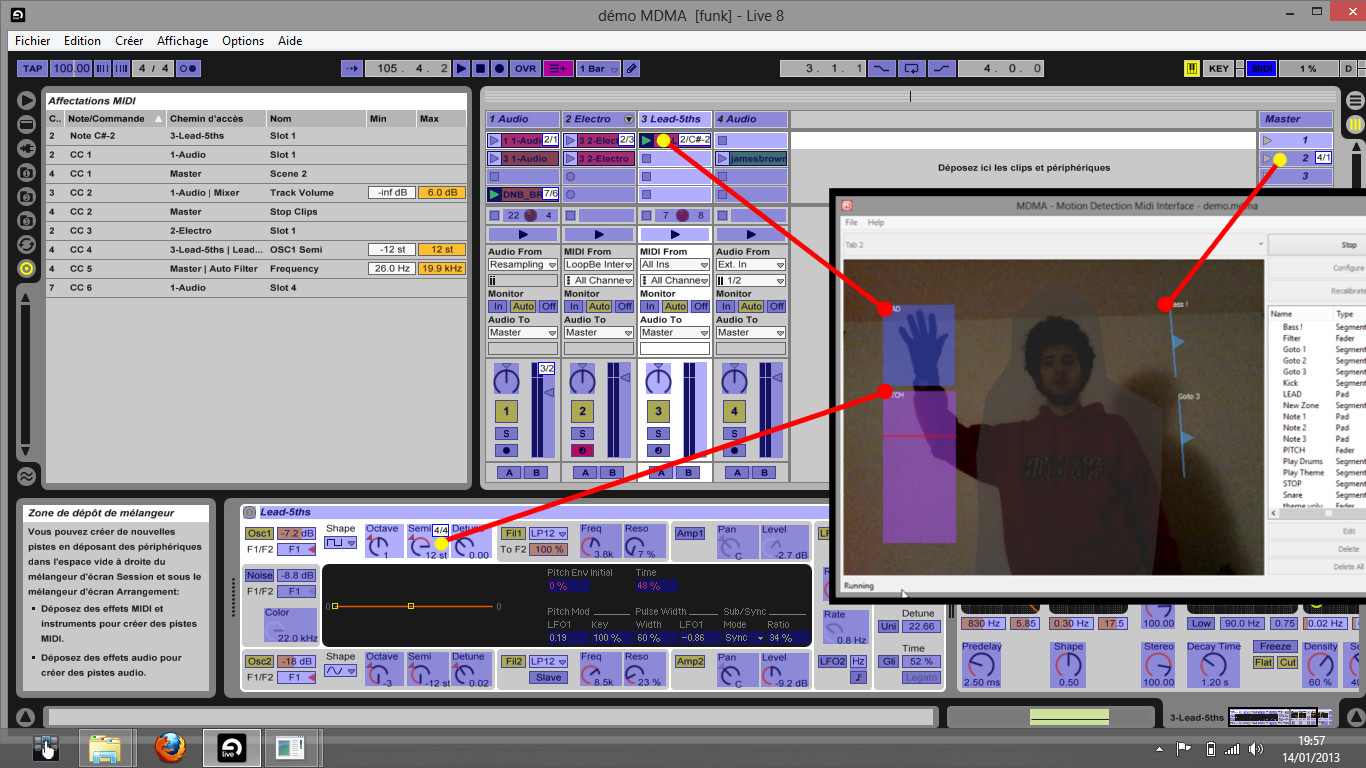
\includegraphics[width=10cm]{mapping}
  \caption{Quelques assignations sous Live}
  \label{live}
\end{figure}
\section{Conclusion}
\par Après quatre mois de travail sur ce projet, nous avons obtenu un programme qui satisfait nos attentes. Nous avons dû faire des choix cruciaux dans sa réalisation, nous avons parfois eu à repenser nos objectifs, et il a fallu une certaine inventivité pour arriver à nous fins. Le résultat final est tout ce que nous avons pu espérer : MDMA est un contrôleur MIDI fonctionnel, totalement configurable, et il détecte étonnamment bien les mouvements de l'utilisateur pour en faire de la musique. 
\par Nous avons fait le choix d'utiliser des gants, de travailler avec une webcam malgré ses défauts... Mais ces choix restent conformes à nos objectifs initiaux, fournir un contrôleur efficace et unique en son genre qui ne demande aucun matériel supplémentaire au musicien, si ce n'est ses propres mains.
\par La communication autour de MDMA nous a révélé l'intérêt que pouvaient porter certains professionnels de la musique à un tel projet. Avec l'essor que connaît actuellement la musique électronique, notre contrôleur a probablement de l'avenir, et il nous reste de nombreuses idées d'améliorations. Des versions Kinect et Leap Motion sont envisagées, et ces périphériques nous permettrons peut-être de mettre au point de nouveaux types de détections, enrichissant encore ce contrôleur.
%% ===================================================================
\end{document}
